\documentclass{article}
\usepackage{amsmath}
\usepackage{mathtools}
\usepackage[a4paper, total={6in, 8in}]{geometry}
\usepackage{amssymb}
\usepackage{color}
\usepackage{lscape}
\usepackage{listings}
\usepackage{xcolor}
\usepackage{float}
\usepackage{fancyhdr}
\pagestyle{fancy}

% Define the header
\fancyfoot[R]{Fernando Urbano}
\renewcommand{\footrulewidth}{0.2pt}

\fancyhead[L]{ECMA 31380 - Causal Machine Learning}
\fancyhead[R]{Homework 2}

\usepackage{graphicx}
\setlength{\parskip}{0.5em}
\setlength{\parindent}{0pt}
\renewcommand{\thesubsection}{\thesection.\alph{subsection}}
\newcommand{\divider}{\vspace{1em}\hrule\vspace{1em}}

\definecolor{codegreen}{rgb}{0,0.6,0}
\definecolor{codegray}{rgb}{0.5,0.5,0.5}
\definecolor{codepurple}{rgb}{0.58,0,0.82}
\definecolor{backcolour}{rgb}{0.95,0.95,0.92}

\lstdefinestyle{Rstyle}{
  backgroundcolor=\color{backcolour},   
  commentstyle=\color{codegreen},
  keywordstyle=\color{blue},
  numberstyle=\tiny\color{codegray},
  stringstyle=\color{codepurple},
  basicstyle=\ttfamily\footnotesize,
  breakatwhitespace=false,         
  breaklines=true,                 
  captionpos=b,                    
  keepspaces=true,                 
  numbers=left,                    
  numbersep=5pt,                  
  showspaces=false,                
  showstringspaces=false,
  showtabs=true,                  
  tabsize=2,
  language=R
}

\title{ECMA 31380 - Causal Machine Learning - Homework 2}
\author{Fernando Rocha Urbano}
\date{Autumn 2024}

% Define colors
\definecolor{codegreen}{rgb}{0,0.6,0}
\definecolor{codegray}{rgb}{0.5,0.5,0.5}
\definecolor{codepurple}{rgb}{0.58,0,0.82}
\definecolor{backcolour}{rgb}{0.95,0.95,0.92}

% Setup the listings package
\lstdefinestyle{mystyle}{
    backgroundcolor=\color{backcolour},   
    commentstyle=\color{codegreen},
    keywordstyle=\color{magenta},
    numberstyle=\tiny\color{codegray},
    stringstyle=\color{codepurple},
    basicstyle=\ttfamily\footnotesize,
    breakatwhitespace=false,         
    breaklines=true,                 
    captionpos=b,                    
    keepspaces=true,                 
    numbers=left,                    
    numbersep=5pt,                  
    showspaces=false,                
    showstringspaces=false,
    showtabs=false,                  
    tabsize=2
}

\newenvironment{colorparagraph}[1]{\par\color{#1}}{\par}
\definecolor{questioncolor}{RGB}{20, 40, 150}
\definecolor{tacolor}{RGB}{200, 0, 0}

\lstset{style=mystyle}

\begin{document}

\maketitle

\begin{colorparagraph}{questioncolor}
\rule{\textwidth}{0.5pt}

\label{q1}\section{Multiple Testing and Heterogeneous Treatment Effects}

We have i.i.d. data from a randomized experiment with a binary treatment \( T \in \{0,1\} \), a continuous outcome of interest \( Y \), a set of binary covariates \( X = (X_1, X_2, \dots, X_d)' \in \{0,1\}^d \) and a set of continuous covariates \( W \in \mathbb{R}^l \). Both \( X \) and \( W \) are pre-treatment and all our usual assumptions are met.

\rule{\textwidth}{0.5pt}
\end{colorparagraph}

\begin{colorparagraph}{questioncolor}
\label{q1a}\subsection{Conditional Average Treatment Effects}
(a) Define the univariate conditional average treatment effects with respect to each \( X_j \) as \( \tau_j(x) = \mathbb{E}[Y(1) - Y(0) \mid X_j = x] \) for \( j \in \{1, \dots, d\} \) and \( x \in \{0, 1\} \). Use a linear regression to propose an estimator for \( \tau_j(x) \) and establish its asymptotic distribution. Provide all necessary regularity conditions. Construct your estimation so that the estimators for \( \tau_j(x) \) and \( \tau_k(x') \) are based on independent data if \( j \neq k \) or \( x \neq x' \).

\rule{\textwidth}{0.5pt}
\end{colorparagraph}

For each \( j \in \{1, \dots, d\} \) and \( x \in \{0,1\} \), define the univariate conditional average treatment effect (CATE) as:
\[
\tau_j(x) = \mathbb{E}[Y(1) - Y(0) \mid X_j = x].
\]
This represents the expected difference in potential outcomes between treated and untreated individuals, conditional on \( X_j = x \).

To estimate \( \tau_j(x) \), a linear regression model is applied to observations where \( X_{ij} = x \):

\[
Y_i = \alpha_{jx} + \tau_j(x) T_i + \beta_{jx}' W_i + \varepsilon_i, \quad \text{for all } i \text{ such that } X_{ij} = x.
\]

In this model:
\begin{itemize}
    \item \( \alpha_{jx} \) is the intercept term specific to \( X_j = x \).
    \item \( \tau_j(x) \) is the coefficient on the treatment indicator \( T_i \), representing the CATE.
    \item \( W_i \) is the vector of continuous covariates.
    \item \( \beta_{jx} \) is the vector of coefficients associated with \( W_i \).
    \item \( \varepsilon_i \) is the error term with zero conditional mean: \( \mathbb{E}[ \varepsilon_i \mid T_i, W_i ] = 0 \).
\end{itemize}
The Ordinary Least Squares (OLS) estimator \( \hat{\tau}_j(x) \) is obtained by fitting this regression model to the data subset where \( X_{ij} = x \).

One could also add $X_{i, -j}$ to the regression, meaning all binary covariates excluding $X_j$. With and without the addition of binary we expect to recover the true CATE from the regression. Adding the covariates should reduce the variance of the estimator.

$$
Y_i = \alpha_{jx} + \tau_j(x) T_i + \gamma_{jx}' X_{i,-j} + \beta_{jx}' W_i + \varepsilon_i, \quad \text{for all } i \text{ such that } X_{ij} = x.
$$

Again, considering the case in which we do not add the other binary covariates:

To ensure that estimators \( \hat{\tau}_j(x) \) and \( \hat{\tau}_k(x') \) are based on independent data when \( j \neq k \) or \( x \neq x' \), we partition the dataset into mutually exclusive subsets \( \{ D_{jx} \} \). Specifically, for each combination of \( j \) and \( x \), we define:
\[
D_{jx} = \{ i : X_{ij} = x, \, \text{and} \, i \in S_{jx} \},
\]
where \( S_{jx} \) is a randomly assigned subset of indices such that:
\[
D_{jx} \cap D_{k x'} = \emptyset \quad \text{whenever} \quad (j, x) \neq (k, x').
\]
By estimating \( \tau_j(x) \) using only data from \( D_{jx} \), different estimators are based on disjoint samples, ensuring their independence.

\textbf{Asymptotic Distribution of the Estimator}

Under suitable regularity conditions, the estimator \( \hat{\tau}_j(x) \) is consistent and asymptotically normal:
\[
\sqrt{n_{jx}} \left( \hat{\tau}_j(x) - \tau_j(x) \right) \xrightarrow{d} N\left( 0, \sigma^2_{jx} \right),
\]
where:
\begin{itemize}
    \item \( n_{jx} \) is the number of observations with \( X_{ij} = x \).
    \item \( \sigma^2_{jx} \) is the asymptotic variance of \( \hat{\tau}_j(x) \), which can be consistently estimated from the regression.
\end{itemize}

The asymptotic result relies on the following regularity conditions:

\begin{enumerate}
    \item Independent and Identically Distributed Sampling: The data \( \{ (Y_i, T_i, X_i, W_i) \}_{i=1}^n \) are i.i.d. draws from the population.
    \item Random Assignment of Treatment: The treatment \( T_i \) is randomly assigned, independent of potential outcomes \( Y(1), Y(0) \) and covariates \( X_i, W_i \).
    \item Finite Fourth Moments: All variables \( Y_i \), \( T_i \), and components of \( W_i \) have finite fourth moments.
    \item Full Rank Condition: The matrix
    \[
    \mathbb{E}\left[ 
    \begin{pmatrix}
    1 \\
    T_i \\
    W_i
    \end{pmatrix}
    \begin{pmatrix}
    1 & T_i & W_i'
    \end{pmatrix}
    \Bigg| X_j = x
    \right]
    \]
    is positive definite.
    \item Zero Conditional Mean of Errors: The error term satisfies \( \mathbb{E}[ \varepsilon_i \mid T_i, W_i ] = 0 \).
\end{enumerate}


\begin{colorparagraph}{questioncolor}
\rule{\textwidth}{0.5pt}

\label{q1b}\subsection{5\% Level Test for \( H_0: \tau_1(1) = 0 \)}
(b) Construct a 5\% level test of \( H_0 : \tau_1(1) = 0 \) versus \( H_1 : \tau_1(1) \neq 0 \) based on the t-statistic from the asymptotic distribution above. Call the test statistic \( t_{11} \). Give the test statistic, its distribution, the critical region, and describe when you reject the null and when you fail to reject. Prove that your test is consistent.

\rule{\textwidth}{0.5pt}
\end{colorparagraph}

The test statistic is constructed using the estimator \( \hat{\tau}_1(1) \) and its estimated standard deviation \( \hat{\sigma}_{11} \):

\[
t_{11} = \frac{\sqrt{n_{11}} \, \hat{\tau}_1(1)}{\hat{\sigma}_{11}},
\]

where:
\begin{itemize}
    \item \( n_{11} \) is the number of observations with \( X_{i1} = 1 \).
    \item \( \hat{\sigma}_{11} \) is a consistent estimator of the asymptotic standard deviation of \( \sqrt{n_{11}} \, \hat{\tau}_1(1) \).
\end{itemize}

Under the null hypothesis \( H_0 \) and the regularity conditions, the test statistic \( t_{11} \) has an asymptotic standard normal distribution:

\[
t_{11} \xrightarrow{d} N(0,1) \quad \text{under } H_0.
\]

For a two-sided test at the 5\% significance level, the critical values are the 2.5th and 97.5th percentiles of the standard normal distribution:

\[
\text{Reject } H_0 \quad \text{if} \quad |t_{11}| > z_{0.975},
\]

where \( z_{0.975} \approx 1.96 \).

The decision rule for it is:

\begin{itemize}
    \item Reject \( H_0 \) if \( |t_{11}| > 1.96 \).
    \item Fail to reject \( H_0 \) if \( |t_{11}| \leq 1.96 \).
\end{itemize}

\textbf{Consistency of the Test}

To prove that the test is consistent, we need to show that under the alternative hypothesis \( H_1: \tau_1(1) \neq 0 \), the probability of rejecting \( H_0 \) approaches 1 as \( n_{11} \to \infty \).

Under \( H_1 \), the test statistic can be expressed as:

\[
t_{11} = \frac{\sqrt{n_{11}} \left( \hat{\tau}_1(1) - \tau_1(1) + \tau_1(1) \right)}{\hat{\sigma}_{11}} = \frac{\sqrt{n_{11}} \left( \hat{\tau}_1(1) - \tau_1(1) \right)}{\hat{\sigma}_{11}} + \frac{\sqrt{n_{11}} \, \tau_1(1)}{\hat{\sigma}_{11}}.
\]

The first term converges in distribution to a standard normal random variable:

\[
\frac{\sqrt{n_{11}} \left( \hat{\tau}_1(1) - \tau_1(1) \right)}{\hat{\sigma}_{11}} \xrightarrow{d} N(0,1).
\]

The second term diverges to infinity because \( \tau_1(1) \neq 0 \) and \( \hat{\sigma}_{11} \) is bounded away from zero:

\[
\frac{\sqrt{n_{11}} \, \tau_1(1)}{\hat{\sigma}_{11}} \to 
\begin{cases}
+\infty, & \text{if } \tau_1(1) > 0, \\
-\infty, & \text{if } \tau_1(1) < 0.
\end{cases}
\]

Therefore, under \( H_1 \), the test statistic \( t_{11} \) diverges in the same direction as \( \tau_1(1) \):

\[
t_{11} \xrightarrow{p} 
\begin{cases}
+\infty, & \text{if } \tau_1(1) > 0, \\
-\infty, & \text{if } \tau_1(1) < 0.
\end{cases}
\]

As a result, the probability of \( |t_{11}| > 1.96 \) approaches 1 under \( H_1 \):

\[
\lim_{n_{11} \to \infty} P\left( |t_{11}| > 1.96 \mid H_1 \right) = 1.
\]

This demonstrates that the test is consistent, as it correctly rejects the null hypothesis with probability approaching 1 when \( \tau_1(1) \neq 0 \).

\begin{colorparagraph}{questioncolor}
\rule{\textwidth}{0.5pt}

\label{q1c}\subsection{5\% Level Test for \( H_0: \tau_1(0) = 0 \)}
(c) Construct a 5\% level test of \( H_0 : \tau_1(0) = 0 \) versus \( H_1 : \tau_1(0) \neq 0 \) based on the t-statistic from the asymptotic distribution above. Call the test statistic \( t_{10} \). Give the test statistic, its distribution, the critical region, and describe when you reject the null and when you fail to reject. Prove that your test is consistent.

\rule{\textwidth}{0.5pt}
\end{colorparagraph}

The test statistic \( t_{10} \) is defined using the estimator \( \hat{\tau}_1(0) \) and its estimated standard error \( \hat{\sigma}_{10} \):

\[
t_{10} = \frac{\sqrt{n_{10}} \, \hat{\tau}_1(0)}{\hat{\sigma}_{10}},
\]

where:

\begin{itemize}
    \item \( n_{10} \) is the number of observations with \( X_{i1} = 0 \).
    \item \( \hat{\sigma}_{10} \) is a consistent estimator of the asymptotic standard deviation of \( \sqrt{n_{10}} \, \hat{\tau}_1(0) \).
\end{itemize}

Under the null hypothesis \( H_0 \) and given the regularity conditions, the test statistic \( t_{10} \) has an asymptotic standard normal distribution:

\[
t_{10} \xrightarrow{d} N(0,1) \quad \text{under } H_0.
\]

For a two-sided test at the 5\% significance level, the critical values correspond to the 2.5th and 97.5th percentiles of the standard normal distribution:

\[
\text{Reject } H_0 \quad \text{if} \quad |t_{10}| > z_{0.975},
\]

where \( z_{0.975} \approx 1.96 \).

The decision rule is given by:

\begin{itemize}
    \item Reject \( H_0 \) if \( |t_{10}| > 1.96 \).
    \item Fail to reject \( H_0 \) if \( |t_{10}| \leq 1.96 \).
\end{itemize}

\textbf{Consistency of the Test}

To prove that the test is consistent, we need to show that under the alternative hypothesis \( H_1: \tau_1(0) \neq 0 \), the probability of rejecting \( H_0 \) approaches 1 as \( n_{10} \to \infty \).

Under \( H_1 \), the test statistic can be expressed as:

\[
t_{10} = \frac{\sqrt{n_{10}} \left( \hat{\tau}_1(0) - \tau_1(0) + \tau_1(0) \right)}{\hat{\sigma}_{10}} = \frac{\sqrt{n_{10}} \left( \hat{\tau}_1(0) - \tau_1(0) \right)}{\hat{\sigma}_{10}} + \frac{\sqrt{n_{10}} \, \tau_1(0)}{\hat{\sigma}_{10}}.
\]

The first term converges in distribution to a standard normal random variable:

\[
\frac{\sqrt{n_{10}} \left( \hat{\tau}_1(0) - \tau_1(0) \right)}{\hat{\sigma}_{10}} \xrightarrow{d} N(0,1).
\]

The second term diverges to infinity because \( \tau_1(0) \neq 0 \) and \( \hat{\sigma}_{10} \) is bounded away from zero:

\[
\frac{\sqrt{n_{10}} \, \tau_1(0)}{\hat{\sigma}_{10}} \to
\begin{cases}
+\infty, & \text{if } \tau_1(0) > 0, \\
-\infty, & \text{if } \tau_1(0) < 0.
\end{cases}
\]

Therefore, under \( H_1 \), the test statistic \( t_{10} \) diverges to infinity in the direction of the sign of \( \tau_1(0) \):

\[
t_{10} \xrightarrow{p}
\begin{cases}
+\infty, & \text{if } \tau_1(0) > 0, \\
-\infty, & \text{if } \tau_1(0) < 0.
\end{cases}
\]

As a result, the probability of \( |t_{10}| > 1.96 \) approaches 1 under \( H_1 \):

\[
\lim_{n_{10} \to \infty} P\left( |t_{10}| > 1.96 \mid H_1 \right) = 1.
\]

Thus, the test is consistent, as it correctly rejects the null hypothesis with probability approaching 1 when \( \tau_1(0) \neq 0 \).

\begin{colorparagraph}{questioncolor}
\rule{\textwidth}{0.5pt}

\label{q1d}\subsection{Probability of False Positives in 5\% Level Tests}
(d) By your own argument from part (a), the tests (b) and (c) are independent, and you just established that they are 5\% level tests. Find the probability that at least one of the tests gives a false positive. What does this tell you about how often you will make mistakes?

\rule{\textwidth}{0.5pt}
\end{colorparagraph}

Given that tests (b) and (c) are independent 5\% level tests, we can compute the probability that at least one test yields a false positive under the global null hypothesis (i.e., both \( H_0: \tau_1(1) = 0 \) and \( H_0: \tau_1(0) = 0 \) are true).

For each test, the probability of not committing a Type I error (i.e., correctly failing to reject \( H_0 \) when it is true) is 95\%:

\[
\mathbb{P}(\text{No False Positive in a Single Test}) = 1 - \alpha = 0.95,
\]

where \( \alpha = 0.05 \) is the significance level of the test.

Since the two tests are independent, the joint probability that neither test yields a false positive is:

\begin{align*}
\mathbb{P}(\text{No False Positives in Both Tests}) &= \mathbb{P}(\text{No False Positive in (b)}) \times \mathbb{P}(\text{No False Positive in (c)}) \\
&= 0.95 \times 0.95 = 0.9025.
\end{align*}

Therefore, the probability that at least one test yields a false positive is:

\[
\mathbb{P}(\text{At Least One False Positive}) = 1 - \mathbb{P}(\text{No False Positives in Both Tests}) = 1 - 0.9025 = 0.0975.
\]

This calculation shows that when conducting two independent tests at the 5\% significance level, the probability of committing at least one Type I error increases to 9.75\%. In other words, even though each test individually has a 5\% chance of yielding a false positive, the combined chance of making a mistake in at least one test is higher due to the multiplicity of tests.

It highlights the multiple testing problem: as the number of independent tests increases, the overall probability of making at least one Type I error also increases. Specifically, for \( m \) independent tests at the same significance level \( \alpha \), the probability of making at least one Type I error is:

\[
\mathbb{P}(\text{At Least One False Positive in } m \text{ Tests}) = 1 - (1 - \alpha)^m.
\]

Applying this to our case with \( m = 2 \) and \( \alpha = 0.05 \):

\[
\mathbb{P}(\text{At Least One False Positive}) = 1 - (0.95)^2 = 1 - 0.9025 = 0.0975.
\]

This increased error rate suggests that, in practice, one should be cautious about the potential for false positives when conducting multiple tests.

\begin{colorparagraph}{questioncolor}
\rule{\textwidth}{0.5pt}

\label{q1e}\subsection{Testing Null Hypothesis for Both Groups}
(e) I would like to test the null hypothesis that the treatment is not effective in both groups,

\[
H_0 : \tau_1(1) = 0 \ \text{and} \ \tau_1(0) = 0,
\]

against the alternative that the treatment is effective for at least one group,

\[
H_a : \tau_1(1) \neq 0 \ \text{or} \ \tau_1(0) \neq 0.
\]

I will reject the null if \( |t_{11}| > c \) or \( |t_{10}| > c \). For what c is a 5\% level test?

\rule{\textwidth}{0.5pt}
\end{colorparagraph}

To determine the critical value \( c \) for a 5\% level test, we will reject the null hypothesis

\[
H_0 : \tau_1(1) = 0 \ \text{and} \ \tau_1(0) = 0,
\]

in favor of the alternative

\[
H_a : \tau_1(1) \neq 0 \ \text{or} \ \tau_1(0) \neq 0,
\]

if \( |t_{11}| > c \) or \( |t_{10}| > c \). This setup ensures that the overall Type I error rate is controlled at 5\%.

Given that \( t_{11} \) and \( t_{10} \) are independent test statistics, each following a standard normal distribution under \( H_0 \), the probability of not rejecting the null hypothesis for both tests is:

\[
P\left( |t_{11}| \leq c \ \text{and} \ |t_{10}| \leq c \ \big| \ H_0 \right) = \left[ P\left( |Z| \leq c \right) \right]^2
\]

where \( Z \sim \mathcal{N}(0,1) \). Since we want the overall probability of at least one rejection to equal 5\%, we set

\[
P\left( |t_{11}| \leq c \ \text{and} \ |t_{10}| \leq c \ \big| \ H_0 \right) = 1 - 0.05 = 0.95
\]

which simplifies to

\[
\left[ P\left( |Z| \leq c \right) \right]^2 = 0.95.
\]

Taking the square root of both sides, we find

\[
P\left( |Z| \leq c \right) = \sqrt{0.95} \approx 0.97468.
\]

Using the cumulative distribution function (CDF) for the standard normal distribution, \( \Phi(c) \), we know that

\[
P\left( |Z| \leq c \right) = 2\Phi(c) - 1,
\]

so

\[
2\Phi(c) - 1 = 0.97468.
\]

Solving for \( \Phi(c) \), we find

\[
\Phi(c) = \frac{1 + 0.97468}{2} \approx 0.98734.
\]

To determine \( c \), we find the value that corresponds to the 98.734th percentile of the standard normal distribution:

\[
c \Phi^{-1}\left( \frac{1 + \sqrt{0.95}}{2} \right) \approx \Phi^{-1}(0.98734) \approx 2.2414
\]

The decision rule becomes:
\begin{itemize}
    \item Reject \( H_0 \) if \( |t_{11}| > c \) or \( |t_{10}| > c \).
    \item Fail to reject \( H_0 \) if both \( |t_{11}| \leq c \) and \( |t_{10}| \leq c \).
\end{itemize}

By setting \( c \approx 2.2414 \), we ensure that the combined test maintains an overall Type I error rate of 5\%, adjusting for the multiple comparisons involved in testing two hypotheses simultaneously.

\begin{colorparagraph}{questioncolor}
\rule{\textwidth}{0.5pt}

\label{q1f}\subsection{Testing Two Restrictions with Fixed Level Test}
(f) The previous part refers to testing two restrictions. What happens to the value of \( c \) as the number of restrictions grows, but the level stays fixed at 5\%? Give an expression for \( c \) (as a function of \( d \)) such that we can test the null that \( \tau_j(x) = 0 \) for all \( j \in \{1, \dots, d\} \) and \( x \in \{0,1\} \).

Notice that we have not even begun to explore subgroup effects in earnest, because the above does not consider any interactions.

\rule{\textwidth}{0.5pt}
\end{colorparagraph}

To determine how the critical value \( c \) changes as the number of restrictions grows while maintaining the overall test level at 5\%, we consider testing the null hypothesis:

\[
H_0 : \tau_j(x) = 0 \quad \text{for all} \quad j \in \{1, \dots, d\}, \quad x \in \{0,1\},
\]

against the alternative:

\[
H_1 : \text{There exists } (j, x) \text{ such that } \tau_j(x) \neq 0.
\]

We have a total of \( m = 2d \) independent test statistics \( t_{jx} \), each corresponding to one of the \( \tau_j(x) \). Each \( t_{jx} \) follows an asymptotic standard normal distribution under \( H_0 \):

\[
t_{jx} \xrightarrow{d} N(0,1) \quad \text{under } H_0.
\]

We reject \( H_0 \) if any of the test statistics exceed the critical value \( c \) in absolute value:

\[
\text{Reject } H_0 \quad \text{if} \quad \max_{j,x} |t_{jx}| > c.
\]

Under \( H_0 \), the test statistics \( t_{jx} \) are independent standard normal variables. We need to find \( c \) such that the overall Type I error rate is 5\%:

\[
P\left( \max_{j,x} |t_{jx}| > c \mid H_0 \right) = 0.05.
\]

The probability that a single test statistic does not exceed \( c \) in absolute value is:

\[
P\left( |t_{jx}| \leq c \right) = 2\Phi(c) - 1,
\]

where \( \Phi(c) \) is the cumulative distribution function (CDF) of the standard normal distribution.

Since the test statistics are independent, the probability that none of them exceeds \( c \) is:

\[
P\left( \max_{j,x} |t_{jx}| \leq c \mid H_0 \right) = \left[ P\left( |t_{jx}| \leq c \right) \right]^m = \left( 2\Phi(c) - 1 \right)^m.
\]

Therefore, the probability of rejecting \( H_0 \) is:

\[
P\left( \text{Reject } H_0 \mid H_0 \right) = 1 - \left( 2\Phi(c) - 1 \right)^m = 0.05.
\]

We solve for \( c \) using the equation:

\[
\left( 2\Phi(c) - 1 \right)^m = 1 - 0.05 = 0.95.
\]

Taking the \( m \)-th root:

\[
2\Phi(c) - 1 = (0.95)^{1/m}.
\]

Solving for \( \Phi(c) \):

\[
\Phi(c) = \frac{1 + (0.95)^{1/m}}{2}.
\]

Therefore, the critical value \( c \) as a function of \( d \) (since \( m = 2d \)) is:

\[
c = \Phi^{-1}\left( \frac{1 + (0.95)^{1/(2d)}}{2} \right).
\]

As the number of restrictions \( d \) increases, the exponent \( 1/(2d) \) decreases, and \( (0.95)^{1/(2d)} \) approaches 1 from below. Consequently, \( \Phi(c) \) approaches 1, and \( c \) increases.

To illustrate, consider the limit as \( d \to \infty \):

\[
\lim_{d \to \infty} (0.95)^{1/(2d)} = (0.95)^{0} = 1,
\]

\[
\lim_{d \to \infty} \Phi(c) = \frac{1 + 1}{2} = 1,
\]

\[
\lim_{d \to \infty} c = \Phi^{-1}(1) = \infty.
\]

This indicates that as the number of restrictions grows, the critical value \( c \) increases without bound, making it increasingly difficult to reject \( H_0 \).

In a example, for a specific value of \( d \), we can compute \( c \). Suppose \( d = 5 \) (so \( m = 10 \)):

\[
(0.95)^{1/10} \approx 0.995,
\]

\[
\Phi(c) = \frac{1 + 0.995}{2} = 0.9975
\]

\[
c = \Phi^{-1}(0.9975) \approx 2.81.
\]

Therefore, with \( d = 5 \), the critical value \( c \) is approximately \( 2.81 \).

In conclusion, as the number of restrictions \( d \) increases, the critical value \( c \) required to maintain the overall test level at 5\% increases according to:

\[
c = \Phi^{-1}\left( \frac{1 + (0.95)^{1/(2d)}}{2} \right).
\]

This relationship shows that controlling the family-wise Type I error rate in multiple testing leads to more stringent criteria for rejection, reflecting the need to account for the increased chance of false positives when conducting many tests simultaneously.

\newpage

\begin{colorparagraph}{questioncolor}
\rule{\textwidth}{0.5pt}

\label{q2}\section{Propensity Score Weighting and ATT Estimation}

Assume that the random variables \( (Y_1, Y_0, T, X')' \in \mathbb{R} \times \mathbb{R} \times \{0, 1\} \times \mathbb{R}^d \) obey \( \{Y_1, Y_0\} \perp T \mid X \). The researcher observes \( (Y, T, X')' \), where \( Y = Y_1 T + Y_0(1 - T) \). Define the propensity score \( p(x) = \mathbb{P}[T = 1 \mid X = x] \) and assume it is bounded inside \( (0,1) \). Define \( \mu_t = \mathbb{E}[Y(t) \mid T = 1] \) and \( \mu_t(x) = \mathbb{E}[Y(t) \mid X = x] \). The average treatment effect on the treated (ATT) is \( \tau = \mu_1 - \mu_0 \).

\rule{\textwidth}{0.5pt}
\end{colorparagraph}

\begin{colorparagraph}{questioncolor}
\label{q2a}\subsection{Balancing Score and Propensity Score}
(a) A function \( f(X) \) is called a balancing score if \( X \perp T \mid f(X) \). Prove that the propensity score is a balancing score.

\rule{\textwidth}{0.5pt}
\end{colorparagraph}

To prove that the propensity score \( p(X) = \mathbb{P}[T = 1 \mid X] \) is a balancing score, we need to show that conditioning on \( p(X) \) renders the covariates \( X \) independent of the treatment assignment \( T \). Meaning:

\[
X \perp T \mid p(X).
\]

We can do that by showing that the conditional distribution of \( X \) given \( T \) and \( p(X) \) is the same as the conditional distribution of \( X \) given \( p(X) \) alone. That is, for all measurable subsets \( A \) of the support of \( X \):

\[
\mathbb{P}[X \in A \mid T = t, p(X) = e] = \mathbb{P}[X \in A \mid p(X) = e], \quad \text{for } t \in \{0,1\}, \ e \in (0,1).
\]

To evaluate \( \mathbb{P}[X \in A \mid T = t, p(X) = e] \), we use Bayes' theorem:

\[
\mathbb{P}[X \in A \mid T = t, p(X) = e] = \frac{\mathbb{P}[T = t \mid X \in A, p(X) = e] \mathbb{P}[X \in A \mid p(X) = e]}{\mathbb{P}[T = t \mid p(X) = e]}.
\]

Since \( p(X) \) is a function of \( X \), conditioning on \( X \) implies that \( p(X) \) is known. Therefore:

\[
\mathbb{P}[T = t \mid X, p(X) = e] = \mathbb{P}[T = t \mid X] = 
\begin{cases}
p(X) = e, & \text{if } t = 1, \\
1 - p(X) = 1 - e, & \text{if } t = 0.
\end{cases}
\]

Thus, for all \( x \) such that \( p(x) = e \):

\[
\mathbb{P}[T = t \mid X = x, p(X) = e] = \mathbb{P}[T = t \mid X = x] = 
\begin{cases}
e, & \text{if } t = 1, \\
1 - e, & \text{if } t = 0.
\end{cases}
\]

Therefore, for \( X \in A \):

\[
\mathbb{P}[T = t \mid X \in A, p(X) = e] = 
\begin{cases}
e, & \text{if } t = 1, \\
1 - e, & \text{if } t = 0.
\end{cases}
\]

Next, we compute \( \mathbb{P}[T = t \mid p(X) = e] \):

\[
\mathbb{P}[T = 1 \mid p(X) = e] = e, \quad \mathbb{P}[T = 0 \mid p(X) = e] = 1 - e.
\]

Now, the numerator and denominator of the expression above are equal:

\[
\frac{\mathbb{P}[T = t \mid X \in A, p(X) = e]}{\mathbb{P}[T = t \mid p(X) = e]} = \frac{e}{e} = 1 \quad \text{or} \quad \frac{1 - e}{1 - e} = 1.
\]

Thus:

\[
\mathbb{P}[X \in A \mid T = t, p(X) = e] = \mathbb{P}[X \in A \mid p(X) = e].
\]

Since the conditional distribution of \( X \) given \( T \) and \( p(X) \) equals the conditional distribution of \( X \) given \( p(X) \) alone, we have established that:

\[
X \perp T \mid p(X).
\]

Therefore, the propensity score \( p(X) \) is indeed a balancing score.

The same can be viewed in:

\[
\mathbb{P}[X \in A \mid T = t, p(X) = e] = \frac{\mathbb{P}[T = t \mid X \in A, p(X) = e] \mathbb{P}[X \in A \mid p(X) = e]}{\mathbb{P}[T = t \mid p(X) = e]}.
\]

As defined above:

$$
\mathbb{P}[T = t \mid \in A, p(X) = e] = \mathbb{P}[T = t \mid p(X) = e]
$$

Substituting in the bayes formula:

\begin{align*}
    \mathbb{P}[X \in A \mid T = t, p(X) = e]
    &= \frac{\mathbb{P}[T = t \mid p(X) = e] \mathbb{P}[X \in A \mid p(X) = e]}{\mathbb{P}[T = t \mid p(X) = e]} \\
    &= \mathbb{P}[X \in A \mid p(X) = e]
\end{align*}

Which agains prove:

\[
X \perp T \mid p(X).
\]

\newpage

\begin{colorparagraph}{questioncolor}
\rule{\textwidth}{0.5pt}

\label{q2b}\subsection{Conditional Independence with Propensity Score}
(b) Prove that \( \{Y_1, Y_0\} \perp T \mid X \) implies \( \{Y(1), Y(0)\} \perp T \mid p(X) \).

\rule{\textwidth}{0.5pt}
\end{colorparagraph}

We are given the conditional independence of the potential outcome. Meaning that, conditional on $X$, the potential outcomes are independent of the treatment assignment $T$.

Furthermore, we are also given the balancing score property from the previous question.

Consider the joint conditional probability conditional on $T$ and $p(X)$:

\[
P[Y_1 \leq y_1, Y_0 \leq y_0 \mid T = t, p(X) = e]
\]

Using the law of total probability, we can express this conditional probability as an integral over  X :

\[
\mathbb{P}[Y_1 \leq y_1, Y_0 \leq y_0 \mid T = t, p(X) = e] = \int \mathbb{P}[Y_1 \leq y_1, Y_0 \leq y_0 \mid T = t, X = x] \mathbb{P}[X = x \mid T = t, p(X) = e] \, dx.
\]

Since $\{Y_1, Y_0\} \perp T \mid X$, we have:

$$
\mathbb{P}[Y_1 \leq y_1, Y_0 \leq y_0 \mid T = t, X = x] = \mathbb{P}[Y_1 \leq y_1, Y_0 \leq y_0 \mid X = x].
$$

From the balancing property  $X \perp T \mid p(X)$ , we have:

$$
\mathbb{P}[X = x \mid T = t, p(X) = e] = \mathbb{P}[X = x \mid p(X) = e].
$$

Applying those two modifications to the integral, we get:

\begin{align*}
    \mathbb{P}[Y_1 \leq y_1, Y_0 \leq y_0 \mid T = t, p(X) = e]
    &= \int \mathbb{P}[Y_1 \leq y_1, Y_0 \leq y_0 \mid T = t, X = x] \mathbb{P}[X = x \mid T = t, p(X) = e] \, dx. \\
    &= \int \mathbb{P}[Y_1 \leq y_1, Y_0 \leq y_0 \mid X = x] \mathbb{P}[X = x \mid p(X) = e] \, dx.
\end{align*}

Using the unconditional probability with respect to $X$:

$$
\mathbb{P}[Y_1 \leq y_1, Y_0 \leq y_0 \mid p(X) = e] = \int \mathbb{P}[Y_1 \leq y_1, Y_0 \leq y_0 \mid X = x] \mathbb{P}[X = x \mid p(X) = e] \, dx.
$$

Thus, 

$$
\mathbb{P}[Y_1 \leq y_1, Y_0 \leq y_0 \mid T = t, p(X) = e] = \mathbb{P}[Y_1 \leq y_1, Y_0 \leq y_0 \mid p(X) = e].
$$

Since the joint probability factors into the product of \( P(Y_1, Y_0 \mid p(X)) \) and \( P(T \mid p(X)) \), we conclude that:

\[
\{Y_1, Y_0\} \perp T \mid p(X).
\]

In conclusion, given \( \{Y_1, Y_0\} \perp T \mid X \) and that the propensity score \( p(X) \) is a balancing score, we have proven that \( \{Y_1, Y_0\} \perp T \mid p(X) \).

\begin{colorparagraph}{questioncolor}
\rule{\textwidth}{0.5pt}

\label{q2c}\subsection{Consistent Estimator for \( \mu_1 \)}
(c) Prove that 

\[
\mu_1 = \mathbb{E}[Y(1) \mid T = 1] = \mathbb{E} \left[ \frac{TY}{\mathbb{E}[T]} \right]
\]

and use this to propose a consistent estimator of \( \mu_1 \). Notice that estimation of the \( \mu_1 \) half of the ATT does not require estimation of \( p(X) \) or \( \mu_0(X) \). Explain why.

\rule{\textwidth}{0.5pt}
\end{colorparagraph}

Given that $Y = Y_1 T + Y_0 (1 - T)$, when $T = 1$, we have $Y = Y_1 = Y(1)$. Therefore, the conditional expectation $\mathbb{E}[Y(1) \mid T = 1]$ is simply the expected value of $Y$ among treated units:

$$
\mu_1 = \mathbb{E}[Y \mid T = 1]
$$

Since $T$ is binary ($T = 1$ or $0$), $T Y$ equals $Y$ when $T = 1$ and $0$ when $T = 0$. Thus:

$$
\mathbb{E}[T Y] = \mathbb{E}[Y \mid T = 1] \cdot \mathbb{P}[T = 1] = \mu_1 \cdot \mathbb{E}[T]
$$

\(T\) acts as an indicator function selecting treated units.

Thus:

$$
\mathbb{E}\left[ \frac{T Y}{\mathbb{E}[T]} \right]
= \frac{\mathbb{E}[TY]}{\mathbb{E}[T]}
= \frac{\mu_1 \mathbb{E}[T]}{\mathbb{E}[T]}
= \mu_1
= \mathbb{E}[Y \mid T = 1]
$$

Now, to construct a consistent estimator of \(\mu_1\), we can use the sample counterparts of \(\mathbb{E}[T Y]\) and \(\mathbb{E}[T]\). Given a random sample \(\{(Y_i, T_i, X_i)\}_{i=1}^n\), the estimator is:
\[
\hat{\mu}_1 = \frac{\frac{1}{n} \sum_{i=1}^n T_i Y_i}{\frac{1}{n} \sum_{i=1}^n T_i} = \frac{\sum_{i=1}^n T_i Y_i}{\sum_{i=1}^n T_i}.
\]

Where we used:

$$
\mathbb{E}[TY] = \frac{1}{n} \sum_{i=1}^n T_i Y_i, \quad
\mathbb{E}[T] = \frac{1}{n} \sum_{i=1}^n T_i
$$

This estimator simplifies to the sample average of \(Y_i\) among treated units:
\[
\hat{\mu}_1 = \frac{1}{n_T} \sum_{i: T_i = 1} Y_i,
\]
where \(n_T = \sum_{i=1}^n T_i\) is the number of treated units.

The estimation of \(\mu_1\) relies solely on observed outcomes \(Y_i\) for individuals with \(T_i = 1\). Under the assumption of unconfoundedness (\(\{Y_1, Y_0\} \perp T \mid X\)) and the fact that treatment assignment is independent of potential outcomes given \(X\), the observed \(Y_i\) for treated units are unbiased estimates of \(Y(1)\) for those units.

Since \(\mu_1 = \mathbb{E}[Y(1) \mid T = 1]\), and we observe \(Y_i = Y(1)\) when \(T_i = 1\), the sample average of \(Y_i\) among treated units consistently estimates \(\mu_1\) without requiring any adjustment for covariates or estimation of the propensity score \(p(X)\).

\begin{itemize}
    \item No Need for \(p(X)\): The propensity score could be used to adjust for differences in covariate distributions between treated and control groups. However, when estimating \(\mu_1\), we are only averaging over the treated group, so there is no imbalance to adjust for.
    \item No Need for \(\mu_0(X)\): The function \(\mu_0(X) = \mathbb{E}[Y(0) \mid X]\) pertains to the control potential outcomes. Since \(\mu_1\) concerns only the treated potential outcomes \(Y(1)\), knowledge of \(\mu_0(X)\) is unnecessary for estimating \(\mu_1\).
\end{itemize}

Under the assumption that the treated units are a random sample from the population of treated individuals, the Law of Large Numbers ensures that:
\[
\hat{\mu}_1 = \frac{1}{n_T} \sum_{i: T_i = 1} Y_i \xrightarrow{p} \mathbb{E}[Y \mid T = 1] = \mu_1.
\]

Therefore, \(\hat{\mu}_1\) is a consistent estimator of \(\mu_1\).

For this statement to be true, the following assumptions must hold:
\begin{itemize}
    \item Random sampling: \(\{(Y_i, T_i)\}_{i=1}^n\) are independent and identically distributed (i.i.d.) observations.
    \item Finite moments: \(\mathbb{E}[|Y_i|] < \infty\), ensuring that the expected value of \(Y_i\) exists and is finite.
    \item Non-Zero probability of treatment: \(\mathbb{P}[T_i = 1] = \pi > 0\), ensuring that there are treated units in the sample.
\end{itemize}

If needed to be more precise in our prove, after expressing the $\hat{\mu}_1$ as the ratio of the sample means, we apply the Weak Law of Large Numbers:

\begin{itemize}
    \item For \(\bar{T Y}\):
    \[
    \bar{T Y} = \frac{1}{n} \sum_{i=1}^n T_i Y_i \xrightarrow{p} \mathbb{E}[T_i Y_i] = \mathbb{E}[T_i Y_i].
    \]
    Since \(T_i Y_i\) are i.i.d. and have finite expectation, WLLN applies.
    \item For \(\bar{T}\):
    \[
    \bar{T} = \frac{1}{n} \sum_{i=1}^n T_i \xrightarrow{p} \mathbb{E}[T_i] = \pi.
    \]
    Again, since \(T_i\) are i.i.d. Bernoulli random variables, WLLN applies.
\end{itemize}

And apply Slutsky's Theorem:

\begin{itemize}
    \item Both \(\bar{T Y} \xrightarrow{p} \mu_1 \cdot \pi\) and \(\bar{T} \xrightarrow{p} \pi\)
    \item Since \(\pi > 0\) (non-zero probability of treatment), and \(\pi\) is a constant, we can apply Slutsky's theorem to the ratio:
    \[
    \hat{\mu}_1 = \frac{\bar{T Y}}{\bar{T}} \xrightarrow{p} \frac{\mu_1 \cdot \pi}{\pi} = \mu_1.
    \]
    Therefore, \(\hat{\mu}_1\) is a consistent estimator of \(\mu_1\).
\end{itemize}

\begin{colorparagraph}{questioncolor}
\rule{\textwidth}{0.5pt}

\label{q2d}\subsection{Estimator for \( \mu_0 \)}
(d) Prove that 

\[
\mu_0 = \frac{1}{\mathbb{E}[T]} \mathbb{E} \left[ \frac{(1 - T)p(X)Y}{(1 - p(X))} \right].
\]

Assume you have access to \( \hat{p}(x) \) that is a uniformly consistent estimator of \( p(x) \). Propose a consistent estimator of \( \mu_0 \).

\rule{\textwidth}{0.5pt}
\end{colorparagraph}

% \begin{colorparagraph}{tacolor}REVIEW NEEDED
%     Would be good to review before delivering it.
% \end{colorparagraph}

To express \(\mu_0\) in terms of \(\mathbb{E}[Y(0) \mid X]\), we start by defining

\[
\mu_0 = \mathbb{E}[Y(0) \mid T = 1].
\]

Using the law of iterated expectations,

\[
\mu_0 = \mathbb{E}_X\left[ \mathbb{E}[Y(0) \mid T = 1, X] \right].
\]

Given the unconfoundedness assumption \(\{Y_1, Y_0\} \perp T \mid X\):

\[
\mathbb{E}[Y(0) \mid T = 1, X] = \mathbb{E}[Y(0) \mid X].
\]

Therefore,

\[
\mu_0 = \mathbb{E}_X\left[ \mathbb{E}[Y(0) \mid X] \right] = \mathbb{E}[ \mathbb{E}[Y(0) \mid X] ].
\]

To relate \(\mathbb{E}[Y(0) \mid X]\) to observable quantities, we use the observed data from untreated units:

\[
\mathbb{E}[Y(0) \mid X] = \mathbb{E}[Y \mid T = 0, X].
\]

However, we need to relate \(\mu_0\) to an expectation over the entire sample, involving both treated and untreated units.

Consider the weighted expectation:

\[
\mathbb{E}\left[ \frac{(1 - T) \, p(X)}{1 - p(X)} \, Y \right].
\]

We can compute its conditional expectation given \(X\):

\[
\mathbb{E}\left[ \frac{(1 - T) \, p(X)}{1 - p(X)} \, Y \Big| X \right] = \frac{p(X)}{1 - p(X)} \, \mathbb{E}\left[ (1 - T) Y \mid X \right].
\]

Since \( (1 - T) Y = (1 - T) Y(0) \), we have:

\[
\mathbb{E}\left[ (1 - T) Y \mid X \right] = \mathbb{E}[ (1 - T) Y(0) \mid X ] = \mathbb{E}[ Y(0) \mid X ] \, \mathbb{P}[ T = 0 \mid X ] = \mathbb{E}[ Y(0) \mid X ] \, [1 - p(X)].
\]

Substituting back,

\[
\mathbb{E}\left[ \frac{(1 - T) \, p(X)}{1 - p(X)} \, Y \Big| X \right] = p(X) \, \mathbb{E}[ Y(0) \mid X ].
\]

Next, take the expectation over \(X\):

\[
\mathbb{E}\left[ \frac{(1 - T) \, p(X)}{1 - p(X)} \, Y \right] = \mathbb{E}\left[ p(X) \, \mathbb{E}[ Y(0) \mid X ] \right].
\]

Recall that \(\mathbb{E}[T] = \mathbb{E}[ p(X) ]\), so

\[
\mathbb{E}\left[ \frac{(1 - T) \, p(X)}{1 - p(X)} \, Y \right] = \mathbb{E}[ p(X) \, \mathbb{E}[ Y(0) \mid X ] ] = \mathbb{E}[T] \, \mu_0.
\]

Solving for \(\mu_0\), we obtain:

\[
\mu_0 = \frac{1}{\mathbb{E}[T]} \, \mathbb{E}\left[ \frac{(1 - T) \, p(X)}{1 - p(X)} \, Y \right].
\]

A consistent estimator of \(\mu_0\) can be constructed given a uniformly consistent estimator \(\hat{p}(X)\) of \( p(X) \) as follows:

\[
\hat{\mu}_0 = \frac{1}{\hat{\pi}_T} \, \frac{1}{n} \sum_{i=1}^n \frac{(1 - T_i) \, \hat{p}(X_i)}{1 - \hat{p}(X_i)} \, Y_i,
\]

where \(\hat{\pi}_T = \frac{1}{n} \sum_{i=1}^n T_i\) is the sample proportion of treated units, which is a consistent estimator of \(\mathbb{E}[T]\).

\begin{itemize}
    \item The sample proportion \(\hat{\pi}_T\) converges in probability to \(\mathbb{E}[T]\) by the Law of Large Numbers.
    \item The weighted sum converges to its expected value because the weights and \(Y_i\) are bounded and the estimator \(\hat{p}(X_i)\) converges uniformly to \(p(X_i)\).
    \item Uniform consistency of \(\hat{p}(X)\) ensures that the denominators \(1 - \hat{p}(X_i)\) must be bounded away from zero, preventing instability in the weights.
\end{itemize}

Therefore, \(\hat{\mu}_0\) is a consistent estimator of \(\mu_0\), utilizing the observed data \((Y_i, T_i, X_i)\) and the estimated propensity scores \(\hat{p}(X_i)\).

As $n \to \infty$, $\hat{\mu}_0$ converges in probability to $\mu_0$.

\begin{colorparagraph}{questioncolor}
\rule{\textwidth}{0.5pt}

\label{q2e}\subsection{Doubly Robust Estimator}
(e) Prove that 

\[
\mu_0 = \frac{1}{\mathbb{E}[T]} \mathbb{E} \left[ T \mu_0(X) + \frac{(1 - T)p(X)(Y - \mu_0(X))}{(1 - p(X))} \right].
\]

Further, prove that this moment condition is "doubly robust," meaning that it still holds even if one of \( p(X) \) or \( \mu_0(X) \) is not correctly specified (or cannot be estimated consistently). Replace \( p(X) \) in the above by some other function \( \tilde{p}(X) \) and show that the equality still holds. Do the same for \( \mu_0(X) \).

\rule{\textwidth}{0.5pt}
\end{colorparagraph}
% \begin{colorparagraph}{tacolor}REVIEW NEEDED
%     Would be good to review before delivering it.
% \end{colorparagraph}

We start from the expression of \(\mu_0\) derived previously. From part (d), we have established that
\[
\mu_0 = \frac{1}{\mathbb{E}[T]} \, \mathbb{E}\left[ \frac{(1 - T) \, p(X) \, Y}{1 - p(X)} \right].
\]

Note that we can decompose \(Y\) into \(\mu_0(X)\) and the residuals.
\[
Y = \mu_0(X) + [Y - \mu_0(X)].
\]

Substituting this into the expression, we get
\[
\mu_0 = \frac{1}{\mathbb{E}[T]} \, \mathbb{E}\left[ \frac{(1 - T) \, p(X) \, \left( \mu_0(X) + [Y - \mu_0(X)] \right)}{1 - p(X)} \right].
\]

Split the expectation into two parts:
\[
\mu_0 = \frac{1}{\mathbb{E}[T]} \left\{ \mathbb{E}\left[ \frac{(1 - T) \, p(X) \, \mu_0(X)}{1 - p(X)} \right] + \mathbb{E}\left[ \frac{(1 - T) \, p(X) \, [Y - \mu_0(X)]}{1 - p(X)} \right] \right\}.
\]

We claim that
\[
\mathbb{E}\left[ \frac{(1 - T) \, p(X) \, \mu_0(X)}{1 - p(X)} \right] = \mathbb{E}[T \, \mu_0(X)].
\]

Since \( T \in \{0,1\} \) and \( \mathbb{P}[T = 1 \mid X] = p(X) \), we have
\[
\mathbb{E}[T \, \mu_0(X)] = \mathbb{E}\left[ \mathbb{E}[T \mid X] \, \mu_0(X) \right] = \mathbb{E}[ p(X) \, \mu_0(X) ].
\]
Similarly,
\[
\mathbb{E}\left[ \frac{(1 - T) \, p(X) \, \mu_0(X)}{1 - p(X)} \right] = \mathbb{E}\left[ \mathbb{E}\left[ \frac{(1 - T) \, p(X)}{1 - p(X)} \Big| X \right] \, \mu_0(X) \right].
\]
But
\[
\mathbb{E}\left[ \frac{(1 - T) \, p(X)}{1 - p(X)} \Big| X \right] = \frac{p(X)}{1 - p(X)} \, \mathbb{E}[1 - T \mid X] = \frac{p(X)}{1 - p(X)} \, (1 - p(X)) = p(X).
\]
Therefore,
\[
\mathbb{E}\left[ \frac{(1 - T) \, p(X) \, \mu_0(X)}{1 - p(X)} \right] = \mathbb{E}[ p(X) \, \mu_0(X) ] = \mathbb{E}[T \, \mu_0(X)].
\]

Using the result from before, we have
\[
\mu_0 = \frac{1}{\mathbb{E}[T]} \left\{ \mathbb{E}[T \, \mu_0(X)] + \mathbb{E}\left[ \frac{(1 - T) \, p(X) \, [Y - \mu_0(X)]}{1 - p(X)} \right] \right\}.
\]

Combining the terms, the expression now becomes
\[
\mu_0 = \frac{1}{\mathbb{E}[T]} \, \mathbb{E} \left[ T \, \mu_0(X) + \frac{(1 - T) \, p(X) \, [Y - \mu_0(X)]}{1 - p(X)} \right].
\]
This completes the proof of the equality.

\textbf{Proof of Double Robustness}

We will show that the above equality holds even if either \( p(X) \) or \( \mu_0(X) \) is misspecified.

\textit{Case 1: \( p(X) \) is Replaced by an Arbitrary Function \( \tilde{p}(X) \)}

Suppose we replace \( p(X) \) with any function \( \tilde{p}(X) \) (not necessarily equal to the true propensity score). We need to show that
\[
\mu_0 = \frac{1}{\mathbb{E}[T]} \, \mathbb{E} \left[ T \, \mu_0(X) + \frac{(1 - T) \, \tilde{p}(X) \, [Y - \mu_0(X)]}{1 - \tilde{p}(X)} \right].
\]
holds as long as \( \mu_0(X) \) is correctly specified.
Consider the expectation
\[
E = \mathbb{E} \left[ T \, \mu_0(X) + \frac{(1 - T) \, \tilde{p}(X) \, [Y - \mu_0(X)]}{1 - \tilde{p}(X)} \right].
\]
Since \( T \in \{0,1\} \), we can write \( E \) as
\[
E = \mathbb{E} \left[ T \, \mu_0(X) \right] + \mathbb{E} \left[ \frac{(1 - T) \, \tilde{p}(X) \, [Y - \mu_0(X)]}{1 - \tilde{p}(X)} \right].
\]

For the first term, we have:
\[
\mathbb{E} \left[ T \, \mu_0(X) \right] = \mathbb{E} \left[ \mathbb{E}[ T \mid X ] \, \mu_0(X) \right] = \mathbb{E} \left[ p(X) \, \mu_0(X) \right].
\]

For the second term, we have:

Since \( \tilde{p}(X) \) is arbitrary, we need to analyze
\[
\mathbb{E} \left[ \frac{(1 - T) \, \tilde{p}(X) \, [Y - \mu_0(X)]}{1 - \tilde{p}(X)} \right].
\]
We can write
\[
\mathbb{E} \left[ \frac{(1 - T) \, \tilde{p}(X) \, [Y - \mu_0(X)]}{1 - \tilde{p}(X)} \right] = \mathbb{E}_{X} \left[ \frac{ \tilde{p}(X) }{ 1 - \tilde{p}(X) } \, \mathbb{E} \left[ (1 - T) [Y - \mu_0(X)] \mid X \right] \right].
\]

But
\[
\mathbb{E} \left[ (1 - T) [Y - \mu_0(X)] \mid X \right] = \mathbb{E} \left[ (1 - T) [Y(0) - \mu_0(X)] \mid X \right].
\]
Given that \( \mathbb{E}[ Y(0) \mid X ] = \mu_0(X) \), and \( \mathbb{E}[ Y(0) - \mu_0(X) \mid X ] = 0 \), we have
\[
\mathbb{E} \left[ (1 - T) [Y - \mu_0(X)] \mid X \right] = (1 - p(X)) \times 0 = 0.
\]
Therefore, the second term is zero regardless of \( \tilde{p}(X) \):
\[
\mathbb{E} \left[ \frac{(1 - T) \, \tilde{p}(X) \, [Y - \mu_0(X)]}{1 - \tilde{p}(X)} \right] = 0.
\]

Thus,
\[
E = \mathbb{E} \left[ p(X) \, \mu_0(X) \right].
\]
Recall that \( \mu_0 = \mathbb{E} [ \mu_0(X) ] \), since \( \mu_0(X) = \mathbb{E}[ Y(0) \mid X ] \) and \( \{ Y_0, Y_1 \} \perp T \mid X \). Therefore,
\[
\mu_0 = \mathbb{E} \left[ \mu_0(X) \right] = \mathbb{E} \left[ p(X) \, \mu_0(X) + [1 - p(X)] \, \mu_0(X) \right] = \mathbb{E} \left[ \mu_0(X) \right].
\]
Since \( E = \mathbb{E} \left[ p(X) \, \mu_0(X) \right] \), we have
\[
E = \mathbb{E} \left[ p(X) \, \mu_0(X) \right] = \mathbb{E} \left[ T \, \mu_0(X) \right].
\]
But we need to account for the scaling factor \( \frac{1}{\mathbb{E}[T]} \). Since \( \mathbb{E}[T] = \mathbb{E} \left[ p(X) \right] \), we have
\[
\mu_0 = \frac{1}{\mathbb{E}[T]} \, \mathbb{E} \left[ T \, \mu_0(X) \right] = \mu_0.
\]
Thus, the equality holds even when \( \tilde{p}(X) \) is arbitrary, provided \( \mu_0(X) \) is correctly specified.

\textit{Case 2: \( \mu_0(X) \) is Replaced by an Arbitrary Function \( \tilde{\mu}_0(X) \)}

Suppose we replace \( \mu_0(X) \) with any function \( \tilde{\mu}_0(X) \), while \( p(X) \) is correctly specified. We need to show that
\[
\mu_0 = \frac{1}{\mathbb{E}[T]} \, \mathbb{E} \left[ T \, \tilde{\mu}_0(X) + \frac{(1 - T) \, p(X) \, [Y - \tilde{\mu}_0(X)]}{1 - p(X)} \right].
\]

Again, consider
\[
E = \mathbb{E} \left[ T \, \tilde{\mu}_0(X) + \frac{(1 - T) \, p(X) \, [Y - \tilde{\mu}_0(X)]}{1 - p(X)} \right].
\]

For the first term:

\[
\mathbb{E} \left[ T \, \tilde{\mu}_0(X) \right] = \mathbb{E} \left[ \mathbb{E}[ T \mid X ] \, \tilde{\mu}_0(X) \right] = \mathbb{E} \left[ p(X) \, \tilde{\mu}_0(X) \right].
\]

For the second term:

\[
\mathbb{E} \left[ \frac{(1 - T) \, p(X) \, [Y - \tilde{\mu}_0(X)]}{1 - p(X)} \right] = \mathbb{E}_{X} \left[ \frac{ p(X) }{ 1 - p(X) } \, \mathbb{E} \left[ (1 - T) [Y - \tilde{\mu}_0(X)] \mid X \right] \right].
\]
Since
\[
\mathbb{E} \left[ (1 - T) [Y - \tilde{\mu}_0(X)] \mid X \right] = [1 - p(X)] \left( \mathbb{E}[ Y(0) \mid X ] - \tilde{\mu}_0(X) \right) = [1 - p(X)] \left( \mu_0(X) - \tilde{\mu}_0(X) \right).
\]
Therefore,
\[
\mathbb{E} \left[ \frac{(1 - T) \, p(X) \, [Y - \tilde{\mu}_0(X)]}{1 - p(X)} \right] = p(X) \, \mathbb{E} \left[ \mu_0(X) - \tilde{\mu}_0(X) \right] = p(X) \left( \mathbb{E}[ \mu_0(X) ] - \mathbb{E}[ \tilde{\mu}_0(X) ] \right).
\]

Adding the two terms,
\[
E = \mathbb{E} \left[ p(X) \, \tilde{\mu}_0(X) \right] + p(X) \left( \mathbb{E}[ \mu_0(X) ] - \mathbb{E}[ \tilde{\mu}_0(X) ] \right) = p(X) \, \mathbb{E}[ \mu_0(X) ].
\]
Since \( \mathbb{E}[T] = \mathbb{E}[ p(X) ] \), we have
\[
\frac{1}{\mathbb{E}[T]} \, E = \frac{ p(X) }{ \mathbb{E}[ p(X) ] } \, \mathbb{E}[ \mu_0(X) ] = \mu_0.
\]
Thus, the equality holds even when \( \tilde{\mu}_0(X) \) is arbitrary, provided \( p(X) \) is correctly specified.


In conclusion, The moment condition
\[
\mu_0 = \frac{1}{\mathbb{E}[T]} \, \mathbb{E} \left[ T \, \tilde{\mu}_0(X) + \frac{(1 - T) \, \tilde{p}(X) \, [Y - \tilde{\mu}_0(X)]}{1 - \tilde{p}(X)} \right]
\]
holds if either \( \tilde{p}(X) = p(X) \) or \( \tilde{\mu}_0(X) = \mu_0(X) \).

This demonstrates the double robustness of the estimator: it remains consistent if either the propensity score model or the outcome model is correctly specified.

\newpage

\begin{colorparagraph}{questioncolor}
\rule{\textwidth}{0.5pt}

\label{q3}\section{Application -- Pricing Experiment}

We have data from a pricing experiment from an online recruiting service. The unit of observation is a customer of this service, which is a firm looking to hire (applicants use the service for free). The firms are charged a fixed price for access to the online recruiting system and its tools. Currently, the price is 99. But they are concerned this price is too low, so they ran an experiment. Arriving customers were randomly assigned a price of either 99 or 249. We observe the decision to either buy the service or not and we observe the \texttt{customerSize} for each firm. The data is in the file \texttt{priceExperiment.csv}.

\rule{\textwidth}{0.5pt}
\end{colorparagraph}

\begin{colorparagraph}{questioncolor}
\label{q3a}\subsection{Regression of Purchase Decision on Price}
(a) Run a regression of the binary outcome \texttt{buy} on the \texttt{price}. Is this regression causal? What do the intercept and slope in this regression represent? Use potential outcomes.

\rule{\textwidth}{0.5pt}
\end{colorparagraph}

We run a regression as:

$$
\text{buy}_i = \beta_0 + \beta_i \times \text{price}_i + \varepsilon_i
$$

\begin{lstlisting}[style=Rstyle, caption=Simple Regression on Price Experiment]
lm(buy ~ price, price_experiment) %>% summary()

"""
Call:
lm(formula = buy ~ price, data = price_experiment)

Residuals:
    Min      1Q  Median      3Q     Max 
-0.2432 -0.2432 -0.1140 -0.1140  0.8860 

Coefficients:
              Estimate Std. Error t value Pr(>|t|)    
(Intercept)  0.3284017  0.0195456  16.802   <2e-16 ***
price       -0.0008611  0.0001039  -8.287   <2e-16 ***
---
Signif. codes:  0 '***' 0.001 '**' 0.01 '*' 0.05 '.' 0.1 ' ' 1

Residual standard error: 0.3788 on 2361 degrees of freedom
Multiple R-squared:  0.02826,	Adjusted R-squared:  0.02785 
F-statistic: 68.67 on 1 and 2361 DF,  p-value: < 2.2e-16
"""

\end{lstlisting}

The estimate parameters are:

$$
\hat{\text{buy}}_i = 0.3284 - 0.0008611 \times \text{price}_i
$$

The intercept $\hat{\beta}_0$ represents the expected value of the variable buy when the price is 0:

$$
\hat{\beta}_0 = \mathbb{E}[\text{buy}_i | \text{price}_i = 0]
$$

We are careful to not say that this is a probability, since it is not bounded between 0 and 1. A big enough price would lead to a negative $\mathbb{E}[\text{buy}_i]$, which does not make sense.

The slope $\beta_1$ captures the change in expectation of purchase for a one-dollar increase in price:

$$
\beta_1 = \dfrac{\Delta \mathbb{E}[\text{buy}_i]}{\Delta \text{price}_i}
$$
    
According to the data, for every additional dollar in price, the expected value of the variable purchase decreases by 0.08611. Meaning that higher prices leads to a lower likelihood of purchase.

Given that this is a RCT, the regression can be interpreted causally. The key reason is that the price was randomly assigned to customers as part of an experiment. Random assignment ensures that the price offered is independent of any customer characteristics or unobserved factors that could influence the purchase decision. This means that any observed difference in the purchase rate between the two price levels can be attributed to the effect of the price itself, not to confounding variables.

With that, we can also estimate the ATE of increasing the price from \$99 to \$249.

Using potential outcome notation:

\begin{itemize}
    \item $Y_i (99)$ is the outcome if offered the price of 99.
    \item $Y_i (249)$ is the outcome if offered the price of 249.
\end{itemize}

The expected conditional:

\begin{itemize}
    \item $\mathbb{E}[Y_i (99)] = 0.3284 - 0.0008611 \times 99 = 0.24315$
    \item $\mathbb{E}[Y_i (249)] = 0.3284 - 0.0008611 \times 249 = 0.11399$ 
\end{itemize}

With that:

$$
\text{ATE} = 0.11399 - 0.24315 = -0.12916
$$

Thus, considering that the treatment is the change of price from \$99 to \$249, the ATE has a negative value of $-0.12916$.

This mean that the increase in price by \$150 reduces the expected value of purchase by approximately 0.1292.

\newpage

\begin{colorparagraph}{questioncolor}
\rule{\textwidth}{0.5pt}

\label{q3b}\subsection{Dummy Variable Regression on Price}
(b) Create a dummy variable indicating the different prices. Regress \texttt{buy} on this variable. Is this regression causal? What do the intercept and slope in this regression represent? Use potential outcomes.

\rule{\textwidth}{0.5pt}
\end{colorparagraph}

We run a regression as:

$$
\text{buy}_i = \beta_0 + \beta_1 \times \text{price\_dummy}_i + \varepsilon_i
$$

\begin{lstlisting}[style=Rstyle, caption=Simple Regression with Dummy on Price Experiment]
price_experiment_with_dummy <- price_experiment %>% 
  mutate(price_dummy = ifelse(price == 249, 1, 0))

lm(buy ~ price_dummy, price_experiment_with_dummy) %>% summary()

"""
Call:
lm(formula = buy ~ price_dummy, data = price_experiment_with_dummy)

Residuals:
    Min      1Q  Median      3Q     Max 
-0.2432 -0.2432 -0.1140 -0.1140  0.8860 

Coefficients:
            Estimate Std. Error t value Pr(>|t|)    
(Intercept)  0.24315    0.01091  22.285   <2e-16 ***
price_dummy -0.12916    0.01559  -8.287   <2e-16 ***
---
Signif. codes:  0 '***' 0.001 '**' 0.01 '*' 0.05 '.' 0.1 ' ' 1

Residual standard error: 0.3788 on 2361 degrees of freedom
Multiple R-squared:  0.02826,	Adjusted R-squared:  0.02785 
F-statistic: 68.67 on 1 and 2361 DF,  p-value: < 2.2e-16
"""
\end{lstlisting}


The estimate parameters are:

$$
\hat{\text{buy}}_i = 0.24315 - 0.12916 \times \text{price\_dummy}_i
$$

The intercept $\hat{\beta}_0$ represents the expected value of the variable buy when the treatment is not applied, meaning the expected value of the variable buy when the price is \$99.

$$
\hat{\beta}_0 = \mathbb{E}[\text{buy}_i | \text{price\_dummy}_i = 0] = \mathbb{E}[\text{buy}_i | \text{price}_i = 99]
$$

The $\hat{\beta}_1$ is the ATE. Meaning the average effect on the buy variable when the treatment is applied.

$$
\text{ATE} = \beta_1 = \mathbb{E}[\text{buy}_i | \text{price\_dummy}_i = 1] - \mathbb{E}[\text{buy}_i | \text{price\_dummy}_i = 0]
$$

Using potential outcome notation:

\begin{itemize}
    \item $Y_i (0)$ is the outcome if offered the price of 99.
    \item $Y_i (1)$ is the outcome if offered the price of 249.
\end{itemize}

\begin{itemize}
    \item $\mathbb{E}[Y_i (0)] = 0.24315$
    \item $\mathbb{E}[Y_i (1)] = 0.24315 - 0.12916 \times 1 = 0.11399$ 
\end{itemize}

The result matches with the previous regression results.

The regression again can be interpreted causally and gives the expected change in the target variable as a consequence of applying or not the treatment.

This interpretation is grounded in the potential outcomes framework, affirming that the observed effect is causal due to the random assignment of prices in the experiment.


\begin{colorparagraph}{questioncolor}
\rule{\textwidth}{0.5pt}

\label{q3c}\subsection{Regression of Revenue on Price Dummy}
(c) Create a variable that measures revenue. Regress this outcome on the dummy variable you just created. Is this regression causal? What do the intercept and slope in this regression represent? Compare explicitly to the previous question. Use potential outcomes.

\rule{\textwidth}{0.5pt}
\end{colorparagraph}

We define:

$$
\text{revenue}_i := \text{price}_i \times \text{buy}_i
$$

We run a regression as:

$$
\text{revenue}_i = \beta_0 + \beta_1 \times \text{price\_dummy}_i + \varepsilon_i
$$

\begin{figure}[H]
\centering
\begin{lstlisting}[style=Rstyle, caption=Simple Regression on Price Experiment]
price_experiment_with_revenue <- price_experiment_with_dummy %>% 
  mutate(revenue = buy * price)

lm(revenue ~ price_dummy, price_experiment_with_revenue) %>% summary()

"""
Call:
lm(formula = revenue ~ price_dummy, data = price_experiment_with_revenue)

Residuals:
   Min     1Q Median     3Q    Max 
-28.38 -28.38 -24.07 -24.07 220.62 

Coefficients:
            Estimate Std. Error t value Pr(>|t|)    
(Intercept)   24.072      1.820  13.226   <2e-16 ***
price_dummy    4.311      2.600   1.658   0.0974 .  
---
Signif. codes:  0 '***' 0.001 '**' 0.01 '*' 0.05 '.' 0.1 ' ' 1

Residual standard error: 63.18 on 2361 degrees of freedom
Multiple R-squared:  0.001163,	Adjusted R-squared:  0.0007402 
F-statistic:  2.75 on 1 and 2361 DF,  p-value: 0.09741
"""
\end{lstlisting}
\end{figure}

We run a regression as:

$$
\text{revenue}_i = 24.072 + 4.311 \times \text{price\_dummy}_i + \varepsilon_i
$$

The regression can again be interpreted causally due to the random assignment of customers.

$\beta_0$ represents the expected revenue for the control group (price equals to \$99). Meaning:

$$
\beta_0 = \mathbb{E}[\text{revenue}_i | \text{price\_dummy}_i = 0] = \mathbb{E}[\text{revenue}_i | \text{price}_i = 99]
$$

The interpretation of the slope $\beta_1$ is the change in expected revenue when moving the price to \$249.

$$
\beta_1 = \mathbb{E}[\text{revenue}_i | \text{price\_dummy}_i = 1] = \mathbb{E}[\text{revenue}_i | \text{price}_i = 249]
$$

Given the positive $4.311$, an increase in price from 99 to 249 increases the expected revenue per customer by approximately \$4.31.

In this case:

\begin{itemize}
    \item $Y_i(0)$ is the revenue if offered the price \$99.
    \item $Y_i(1)$ is the revenue if offered the price \$249.
\end{itemize}

Due to the assumptions previously specified, we can also view the $\beta_1$ as the ATE.

$$
\text{ATE} = \mathbb{E}[Y_i(1) - Y_i(0)] = \beta_1 = 4.311
$$

In the previous question, we saw that expected value of $\text{buy}_i$ decreases from 24.32\% to 11.40\%. 

Despite the decrease in purchase expectation, the current regression shows that expected revenue increases when the price is raised from \$99 to \$249. This is due to the higher price per purchase compensating for the lower purchase rate.

The $\beta_1$ can be viewed in the lens of purchase probability and increase price:

$$
\mathbb{E}[\text{revenue}_i | \text{price}_i = 99] = \mathbb{P}[\text{buy}_i | \text{price}_i = 99] \times 99 = 24.072
$$

$$
\mathbb{E}[\text{revenue}_i | \text{price}_i = 249] = \mathbb{P}[\text{buy}_i | \text{price}_i = 249] \times 249 = 28.383
$$

Nonetheless, it is worth to mention that the $\beta_1$ is only significant at 10\% (in 3.d we use robust errors, leading to $\text{p-value}$ even higher than 10\%).
This suggests that while there is an indication that increasing the price may lead to higher revenue, the evidence is not strong enough. The addition of other important variables and their relationship to the treatment might help increase the certainty.

\begin{colorparagraph}{questioncolor}
\rule{\textwidth}{0.5pt}

\label{q3d}\subsection{Statistical Significance of Price Effects}
(d) At the 95\% level, are the effects in parts (b) and (c) statistically significant? Justify your choice of standard errors.

\rule{\textwidth}{0.5pt}
\end{colorparagraph}

Part (b):

\begin{itemize}
    \item Coefficient of price dummy: -0.12916.
    \item Standard Error: 0.01559.
    \item t-value: -8.287.
    \item p-value: $< 2e-16$.
\end{itemize}

At the 95 \% confidence level, the effect of price\_dummy on the probability of purchase (buy) is statistically significant.
The p-value is significantly less than 0.05, indicating strong evidence against the null hypothesis of no effect. Therefore, we reject the null hypothesis and conclude that changing the price from \$99 to \$249 has a statistically significant impact on the purchase decision.

Part (c):

\begin{itemize}
    \item Coefficient of price dummy: 4.311.
    \item Standard Error: 2.600.
    \item t-value: 1.658.
    \item p-value: 0.0974.
\end{itemize}

At the 95\% confidence level, the effect of price\_dummy on expected revenue is not statistically significant. The p-value of 0.0974 exceeds the conventional threshold of 0.05, meaning we do not have sufficient evidence to reject the null hypothesis of no effect. Therefore, we cannot conclude that changing the price from \$99 to \$249 has a statistically significant impact on expected revenue at the 95\% confidence level.

In both regressions, the nature of the data suggests that the error terms may exhibit heteroskedasticity—that is, the variance of the errors is not constant across observations. Here's why:

Part (b):

\begin{itemize}
    \item The outcome variable buy is binary (takes the value 0 or 1). In a linear probability model (LPM), where a binary dependent variable is regressed on independent variables using OLS, the error terms are heteroskedastic by construction.
    \item The variance of the error term depends on the predicted probability, violating the homoskedasticity assumption of OLS.
    \item Use heteroskedasticity-robust standard errors to obtain consistent estimates of the standard errors for hypothesis testing.
\end{itemize}

Part (c):

\begin{itemize}
    \item The revenue variable is calculated as $\text{revenue}_i := \text{buy}_i \times \text{price}_i$. Since buy is binary and price varies, the variance of revenue is likely to differ across observations.
    \item Customers who do not purchase generate zero revenue, while those who purchase contribute revenue equal to the price they pay (\$99 or \$249). This leads to heteroskedasticity in the error terms. The assumption of homoskedasticity is violated, potentially biasing the standard errors.
    \item Again, use heteroskedasticity-robust standard errors to obtain valid inference.
\end{itemize}

We run the regressions again using robust errors:

\begin{figure}[H]
\centering
\begin{lstlisting}[style=Rstyle, caption=Simple Dummy Regression on Price Experiment with Robust Errors]
library(estimatr)

# For Part (b)
model_buy_robust <- lm_robust(buy ~ price_dummy, data = price_experiment_with_dummy, se_type = "HC1")
summary(model_buy_robust)

"""
Call:
lm_robust(formula = buy ~ price_dummy, data = price_experiment_with_dummy, 
    se_type = "HC1")

Standard error type:  HC1 

Coefficients:
            Estimate Std. Error t value  Pr(>|t|) CI Lower CI Upper   DF
(Intercept)   0.2432    0.01236  19.667 7.193e-80   0.2189  0.26740 2361
price_dummy  -0.1292    0.01550  -8.335 1.297e-16  -0.1596 -0.09878 2361

Multiple R-squared:  0.02826 ,	Adjusted R-squared:  0.02785 
F-statistic: 69.47 on 1 and 2361 DF,  p-value: < 2.2e-16
"""
\end{lstlisting}
\end{figure}

\begin{figure}[H]
\centering
\begin{lstlisting}[style=Rstyle, caption=Simple Revenue Dummy Regression on Price Experiment with Robust Errors]
    library(estimatr)
# For Part (c)
model_revenue_robust <- lm_robust(revenue ~ price_dummy, data = price_experiment_with_revenue, se_type = "HC1")
summary(model_revenue_robust)

"""
Call:
lm_robust(formula = revenue ~ price_dummy, data = price_experiment_with_revenue, 
    se_type = "HC1")

Standard error type:  HC1 

Coefficients:
            Estimate Std. Error t value  Pr(>|t|) CI Lower CI Upper   DF
(Intercept)   24.072      1.224   19.67 7.193e-80  21.6720   26.472 2361
price_dummy    4.311      2.629    1.64 1.011e-01  -0.8436    9.466 2361

Multiple R-squared:  0.001163 ,	Adjusted R-squared:  0.0007402 
F-statistic:  2.69 on 1 and 2361 DF,  p-value: 0.1011
"""
\end{lstlisting}
\end{figure}

Part (b):
\begin{itemize}
    \item Without Robust Errors: p-value $< 2 \times 10^{-16}$
    \item With Robust Errors: p-value $1.297 \times 10^{-16}$
\end{itemize}

In part (b), the p-value shows the maintainance of significance at 5\%, and the robust standard errors have minimal impact on the inference.

Part (c):
\begin{itemize}
    \item Without Robust Errors: p-value $0.0974$
    \item With Robust Errors: p-value $0.1011$
\end{itemize}

In part (c), The effect is not statistically significant at the 95\% level in both cases. Thus, there is insignicant evidence at 95\% CI to conclude that raising the price from \$99 to \$249 increases expected revenue.

\begin{colorparagraph}{questioncolor}
\rule{\textwidth}{0.5pt}

\label{q3e}\subsection{Price Recommendation for the Service}
(e) Should the firm stick with 99 or switch to 249? Justify your answer using the results from what you've done so far.

\rule{\textwidth}{0.5pt}
\end{colorparagraph}

Our models show that there is a significant estimate of decrease in "probability" of purchase in the model (3.b). On the other hand, the parameter related to the increase in revenue as a consequence of increase in prices is not significant. This could lead one to think that is not in the firm best interest to increase prices. Nonetheless, this idea is incorrect.

The actual result should be a consequence of decision theory and not necessarily of inference. Having a positive estimate for the coefficient in prices to revenue states that, on average, we should expect the revenue to increase conditioning on increasing prices from \$99 to \$249. Thus, because the $\hat{\beta}$ follows a normal distribution, there is more than 50\% probability that an increase in prices generates an increase in revenue and a positive expected value for revenue increase (using price as \$249).

Thus, the best decision is to increase the prices (discussed during TA section).

\begin{colorparagraph}{questioncolor}
\rule{\textwidth}{0.5pt}

The data includes a variable \texttt{customerSize} that gives the size of the customer firm (remember, the customers of this business are themselves firms). The sizes are ranked 0, 1, 2, for small, medium, and large firms.

\label{q3f}\subsection{CATE Estimation by Firm Size}
(f) Using a \emph{single} regression (e.g., one \texttt{lm()} command), estimate the revenue effect for each firm size individually. That is, obtain estimates of the CATEs \( \tau(x) = \mathbb{E}[Y(1) - Y(0) \mid X = x] \), for \( x = 0, 1, 2 \). Verify your answer manually using a difference in means for each group. Does this pattern make sense to you?

\rule{\textwidth}{0.5pt}
\end{colorparagraph}

\begin{figure}[H]
\centering
\begin{lstlisting}[style=Rstyle, caption=Revenue Effect on Different Firm Sizes]
price_experiment_with_revenue_and_customer <- price_experiment_with_revenue %>% 
  mutate(customerSize = as.factor(customerSize))

model_revenue_customer <- lm(revenue ~ price_dummy * customerSize, data = price_experiment_with_revenue_and_customer)

model_revenue_customer %>% summary()

"""
Call:
lm(formula = revenue ~ price_dummy * customerSize, data = price_experiment_with_revenue_and_customer)

Residuals:
   Min     1Q Median     3Q    Max 
-42.86 -25.84 -25.71 -17.82 223.29 

Coefficients:
                          Estimate Std. Error t value Pr(>|t|)    
(Intercept)                25.8393     2.0174  12.808   <2e-16 ***
price_dummy                -0.1273     2.8969  -0.044   0.9649    
customerSize1              -8.0193     6.6206  -1.211   0.2259    
customerSize2             -10.3706     5.9274  -1.750   0.0803 .  
price_dummy:customerSize1  16.6522     9.0792   1.834   0.0668 .  
price_dummy:customerSize2  27.5193     8.4881   3.242   0.0012 ** 
---
Signif. codes:  0 '***' 0.001 '**' 0.01 '*' 0.05 '.' 0.1 ' ' 1

Residual standard error: 63.06 on 2357 degrees of freedom
Multiple R-squared:  0.006748,	Adjusted R-squared:  0.004641 
F-statistic: 3.202 on 5 and 2357 DF,  p-value: 0.006935
"""
\end{lstlisting}
\end{figure}

\begin{figure}[H]
\centering
\begin{lstlisting}[style=Rstyle, caption=Difference in Means by Customer Size]
mean_revenue_by_group <- price_experiment_with_revenue_and_customer %>%
  group_by(customerSize, price_dummy) %>%
  summarise(mean_revenue = mean(revenue), .groups = 'drop')

difference_in_means <- mean_revenue_by_group %>%
  pivot_wider(names_from = price_dummy, values_from = mean_revenue, names_prefix = "price_") %>%
  mutate(cate = price_1 - price_0)

print(difference_in_means)

"""
# A tibble: 3 x 4
  customerSize price_0 price_1   cate
  <fct>          <dbl>   <dbl>  <dbl>
1 0               25.8    25.7 -0.127
2 1               17.8    34.3 16.5  
3 2               15.5    42.9 27.4
"""
\end{lstlisting}
\end{figure}

We performed a regression of \texttt{revenue} on \texttt{price\_dummy}, \texttt{customerSize}, and their interaction. The regression equation is:

\begin{align*}
    \text{revenue}_i =& \ \beta_0 + \beta_1 \times \text{price\_dummy}_i + \beta_2 \times \text{customerSize1}_i \\ &+ \beta_3 \times \text{customerSize2}_i + \beta_4 \times (\text{price\_dummy}_i \times \text{customerSize1}_i) \\ &+ \beta_5 \times (\text{price\_dummy}_i \times \text{customerSize2}_i) + \varepsilon_i
\end{align*}

The CATE for each firm size is calculated as the difference in expected revenue between the higher price (\$249) and the lower price (\$99), conditional on firm size.

Small Firms (customerSize = 0):

\begin{align*}
    \tau(0) &= E[\text{revenue} \mid \text{price\_dummy} = 1, \text{customerSize} = 0] - E[\text{revenue} \mid \text{price\_dummy} = 0, \text{customerSize} = 0] \\
    &= \beta_1 = -0.1273475
\end{align*}

Medium Firms (customerSize = 1):

\[
\tau(1) = \beta_1 + \beta_4 = -0.1273 + 16.6522 = 16.5248276
\]

Large Firms (customerSize = 2):

\[
\tau(2) = \beta_1 + \beta_5 = -0.1273 + 27.5193 = 27.3919057
\]

The mean revenues for each combination of \texttt{customerSize} and \texttt{price\_dummy} are:

\[
\begin{array}{l c c}
\text{customerSize} & \text{price\_dummy} & \text{mean\_revenue} \\
0 \,(\text{Small}) & 0 & 25.8393 \\
0 \,(\text{Small}) & 1 & 25.7120 \\
1 \,(\text{Medium}) & 0 & 17.8200 \\
1 \,(\text{Medium}) & 1 & 34.3449 \\
2 \,(\text{Large}) & 0 & 15.4688 \\
2 \,(\text{Large}) & 1 & 42.8606 \\
\end{array}
\]

Calculating CATEs:
\[
\begin{array}{l c}
\text{Small Firms:} & \tau(0) = 25.7120 - 25.8393 = -0.1273475 \\
\text{Medium Firms:} & \tau(1) = 34.3449 - 17.8200 = 16.5248276 \\
\text{Large Firms:} & \tau(2) = 42.8897 - 15.4688 = 27.3919057 \\
\end{array}
\]

\begin{itemize}
    \item Small Firms (CATE: -0.1273): Increasing the price from \$99 to \$249 has virtually no effect on the expected revenue from small firms, as evidenced by the non-significant coefficient \(\beta_1\).
    \item Medium Firms (CATE: 16.5249): Increasing the price significantly increases expected revenue for medium firms, with the interaction term \(\beta_4\) being marginally significant at the 10\% level.
    \item Large Firms (CATE: 27.392): The price increase substantially boosts revenue for large firms, with the interaction term \(\beta_5\) showing strong significance (\(p = 0.0012\)).
\end{itemize}

The pattern aligns with economic intuition:

\begin{itemize}
    \item Small firms are likely more price-sensitive due to limited budgets, leading to no significant change in revenue with the price increase.
    \item Medium firms, while somewhat price-conscious, show a moderate increase in revenue when the price rises.
    \item Large firms are less price-sensitive and more likely to pay higher prices for valuable services, resulting in a substantial revenue increase when the price is raised.
\end{itemize}

This pattern implies that the firm could benefit from a differential pricing strategy, potentially implementing tiered pricing to maximize revenue across different customer segments.

\begin{colorparagraph}{questioncolor}
\rule{\textwidth}{0.5pt}

\label{q3g}\subsection{Optimal Pricing Strategy}
(g) Using these results, decide on the optimal pricing strategy to maximize revenue when the service can charge different prices to different customers based on their size. We are imagining that when a firm goes to the service, they first fill out several questions, including their firm size, and then are shown a price based on these answers. (This is known as third-degree price discrimination.)

\rule{\textwidth}{0.5pt}
\end{colorparagraph}

We should use the results from the previous CATE analysis for each firm size segment: small, medium, and large.

The regression and difference-in-means analysis in part (f) suggest that different firm sizes respond differently to price changes. Specifically:

Small Firms (customerSize = 0): keep price at \$99.
\begin{itemize}
    \item The CATE estimate for small firms is approximately zero (\(-0.1273\)), indicating that raising the price from \$99 to \$249 has a negligible impact on revenue for this segment.
\end{itemize}

Medium Firms (customerSize = 1): increase price to \$249.
\begin{itemize}
    \item The CATE for medium firms is positive and moderately large (\(16.5249\)), suggesting that a price increase significantly raises revenue for this segment.
\end{itemize}

Large Firms (customerSize = 2): increase price to \$249.
\begin{itemize}
    \item The CATE for large firms is the highest among the segments (\(27.392\)), indicating a strong positive revenue effect from the price increase.
\end{itemize}

This pricing strategy aligns with the principles of third-degree price discrimination, where different customer segments are charged different prices based on their price sensitivity and ability to pay.

Although third-degree price discrimination can maximize revenue, one should take care to clearly communicate the added value that justifies the higher prices for larger firms. If this is not done properly, there might be a decrease in customer satisfaction.

\begin{colorparagraph}{questioncolor}
\rule{\textwidth}{0.5pt}

\label{q3h}\subsection{Revenue Maximization Potential}
(h) Can the recruiting service improve its revenue? By how much? (\textit{Careful computing the revenue from your strategy. When using the data, think about which observations were exposed to which price, and how many of each type of firm you have.})

\rule{\textwidth}{0.5pt}
\end{colorparagraph}

This question can be answered in one of two ways:

\textbf{Maximizing Revenue for the Population}

Assuming that this sample is representative of the overall population, we can extrapolate results. In such case, we should use the expected values of the model regardless of having observed or not the desired values.

\begin{align*}
    \mathbb{E}[\text{Sample Revenue}] =&
    \sum_{j = 1}^{n_0} \mathbb{E}[Y_j(0)] \quad \text{(customerSize = 0)} \\
    & + \sum_{k = 1}^{n_1} \mathbb{E}[Y_k(1)] \quad \text{(customerSize = 1)} \\
    & + \sum_{i = 1}^{n_2} \mathbb{E}[Y_i(1)] \quad \text{(customerSize = 2)} \\
\end{align*}

\begin{figure}[H]
\centering
\begin{lstlisting}[style=Rstyle, caption=Difference in Means by Customer Size]
expected_revenue_optimal_solution <- tibble(
  best_exp_revenue_small_firms,
  best_exp_revenue_medium_firms,
  best_exp_revenue_large_firms
) %>% 
  t() %>% 
  data.frame() %>% 
  rownames_to_column() %>% 
  tibble() %>% 
  purrr::set_names(c("firm_size", "best_strategy")) %>% 
  mutate(firm_size = c("small", "medium", "large")) %>% 
  mutate(customerSize = c(0, 1, 2)) %>% 
  inner_join(
    price_experiment_with_revenue %>% 
      group_by(customerSize) %>% 
      count(),
    by = "customerSize"
  ) %>% 
  select(-customerSize) %>% 
  mutate(expected_revenue = best_strategy * n)

expected_revenue_optimal_solution

"""
# A tibble: 3 x 4
  firm_size best_strategy     n expected_revenue
  <chr>             <dbl> <int>            <dbl>
1 small              25.8  1897           49017.
2 medium             34.3   216            7418.
3 large              42.9   250           10715.
"""
\end{lstlisting}
\end{figure}

Thus, we can see that the recruiting service can improve its revenue.

Considering the optimal strategy:
\begin{itemize}
    \item Small firms pay \$99, totaling \$49,017.16.
    \item Medium firms pay \$249, totaling \$7418.48.
    \item Big firms pay \$249, totaling \$10715.16.
\end{itemize}

In total, the expected revenue is \$67150.81. An increase of 8.53\% compared to the current revenue (\$61875.00).

Therefore, the optimal strategy is expected to increase revenue by 8.53\% in the population considering that the sample is a good representation of the overall population.

I believe that the question should be answered considering the populational perspective. If necessary, we can also use the sample perspective, aiming to maximize revenue only within the sample.

\textbf{Maximizing Revenue in Sample}

In the sample, $Y(0)$ is observed for the control observations and $Y(1)$ is observed for the treatment observations.
Therefore, for the control observations, we can consider the $Y_i$ instead of $\mathbb{E}[Y(0)]$ given by the model, and, for the treatment observations, we can consider the $Y_i$ instead of $\mathbb{E}[Y(1)]$.

Considering the optimal pricing strategy outlined in (3.g):

\begin{align*}
    \mathbb{E}[\text{Sample Revenue}] =& \sum_{j = 1}^{n_0} (1 - t_j) \times Y_j
    + \sum_{j = 1}^{n_0} t_j \times \mathbb{E}[Y_j(0)] \quad \text{(customerSize = 0)} \\
    & + \sum_{k = 1}^{n_1} (1 - t_k) \times \mathbb{E}[Y_k(0)]
    + \sum_{k = 1}^{n_1} t_k \times Y_k \quad \text{(customerSize = 1)} \\
    & + \sum_{i = 1}^{n_2} (1 - t_i) \times \mathbb{E}[Y_i(0)]
    + \sum_{i = 1}^{n_2} t_i \times Y_i \quad \text{(customerSize = 2)}
\end{align*}

In such a case, one could argue that the optimal strategy would even be more granular:
\begin{itemize}
    \item If a company has received the treatment and bought it, keep it with \$ 249 price.
    \item If a company has not received the treatment and bought it, change the price if the expected value with the treatment is higher than the observed revenue.
    \item If the company has not bought, give it the treatment if it had not received before and vice-versa (considering that there is no negative revenue).
\end{itemize}

\begin{colorparagraph}{questioncolor}
\rule{\textwidth}{0.5pt}

\label{q3i}\subsection{Computing the Plug-in Estimator of the ATE}
(i) The law of iterated expectations says that the ATE obeys

\begin{align*}
    \tau &= \mathbb{E}[\tau(X)] \\
    & = \mathbb{E}[Y(1) - Y(0) \mid X = 0]\mathbb{P}[X = 0] \\
    &\quad + \mathbb{E}[Y(1) - Y(0) \mid X = 1]\mathbb{P}[X = 1] \\
    &\quad + \mathbb{E}[Y(1) - Y(0) \mid X = 2]\mathbb{P}[X = 2].
\end{align*}

Use this and your single regression to compute plug-in estimator of the ATE:

\[
\hat{\tau} = \hat{\tau}(0)\hat{\mathbb{P}}[X = 0] + \hat{\tau}(1)\hat{\mathbb{P}}[X = 1] + \hat{\tau}(2)\hat{\mathbb{P}}[X = 2].
\]

Why does this value not match what you found in part (c)? Explain rigorously and propose a different way of aggregating data from each value of \( X \) so that you obtain exactly the answer in part (c).

\rule{\textwidth}{0.5pt}
\end{colorparagraph}

From part (f), we have the estimates of \(\hat{\tau}(x)\) for each firm size:

\[
\begin{aligned}
\hat{\tau}(0) &= -0.1273, \\
\hat{\tau}(1) &= 16.5249, \\
\hat{\tau}(2) &= 27.392.
\end{aligned}
\]

The proportions of each firm size are:

\[
\begin{aligned}
\hat{\mathbb{P}}[X = 0] &= 0.803, \\
\hat{\mathbb{P}}[X = 1] &= 0.0914, \\
\hat{\mathbb{P}}[X = 2] &= 0.106.
\end{aligned}
\]

Now, compute the plug-in estimator \(\hat{\tau}\):

\[
\begin{aligned}
\hat{\tau} &= \hat{\tau}(0) \times \hat{\mathbb{P}}[X = 0] + \hat{\tau}(1) \times \hat{\mathbb{P}}[X = 1] + \hat{\tau}(2) \times \hat{\mathbb{P}}[X = 2] \\
&= (-0.1273) \times 0.803 + 16.5249 \times 0.0914 + 27.392 \times 0.106.
\end{aligned}
\]

Calculate each term:

1. For \(X = 0\):

\[
(-0.1273) \times 0.803 = -0.1022337.
\]

2. For \(X = 1\):

\[
16.5249 \times 0.0914 = 1.5105217.
\]

3. For \(X = 2\):

\[
27.392 \times 0.106 = 2.8980010.
\]

Sum of the terms:

\[
\hat{\tau} = -0.1022337 + 1.5105217 + 2.8980010 = 4.306289.
\]

In part (c), the estimated effect of \(\text{price\_dummy}\) on \(\text{revenue}\) from the regression was:

\[
\hat{\beta}_1 = 4.311221.
\]

The plug-in estimator and the ATE do not match exactly due to the difference in sample probability of being treated.

In the data:

\begin{table}[H]
    \centering
    \begin{tabular}{|c|c|c|c|c|}
    \hline
    \textbf{customerSize} & \textbf{Nº} & \textbf{\% of Total Treated}
    & \textbf{\% of Total Control} & \textbf{\% Total} \\
    \hline
    0 & 1897 & 79.4\% & 81.1\% & 80.3\% \\
    1 & 216 & 10.0\% & 8.3\% & 9.1\% \\
    2 & 250 & 10.5\% & 10.6\% & 10.6\% \\
    \hline
    \textbf{Total} & 2363 & 100\% & 100\% & 100\% \\
    \hline
    \end{tabular}
    \caption{\% of Total Treatment and Control in Each Group}
    \label{tab:earnings_distribution}
\end{table}

The \texttt{customerSize} $= 0$ contains 79.4\% of the treated firms and 81.1\% of the control firms.
The same difference is evident for \texttt{customerSize} $= 1$. While small, the differences in distribution of treated by firm size leads the plug-in estimator to provide a diverging result when compared to the ATE. We can fix that by accounting for those probabilities when weighting the CATE.

Looking at the formula previously specified:

\begin{align*}
    \tau &= \mathbb{E}[\tau(X)] \\
    & = \mathbb{E}[Y(1) - Y(0) \mid X = 0]\mathbb{P}[X = 0] \\
    &\quad + \mathbb{E}[Y(1) - Y(0) \mid X = 1]\mathbb{P}[X = 1] \\
    &\quad + \mathbb{E}[Y(1) - Y(0) \mid X = 2]\mathbb{P}[X = 2] \\
    & = \mathbb{E}[Y(1) \mid X = 0] \mathbb{P}[X = 0] - \mathbb{E}[Y(0) \mid X = 0] \mathbb{P}[X = 0] \\
    &\quad + \mathbb{E}[Y(1) \mid X = 1] \mathbb{P}[X = 1] - \mathbb{E}[Y(0) \mid X = 1] \mathbb{P}[X = 1] \\
    &\quad + \mathbb{E}[Y(1) \mid X = 2] \mathbb{P}[X = 2] - \mathbb{E}[Y(0) \mid X = 2] \mathbb{P}[X = 2] 
\end{align*}

The formula considers that the probability of having $\mathbb{E}[Y(1) \mid X = 0]$ equals $\mathbb{E}[Y(0) \mid X = 0]$. Nonetheless, it does not match the actual distribution of our sample. In order to make it work properly, we need to adjust by the probabilities in treatment and control:

\begin{align*}
    \hat{\tau} &= 
    \hat{\mathbb{E}}[Y(1) \mid X = 0] \hat{\mathbb{P}}[X = 0 \mid T = 1] - \hat{\mathbb{E}}[Y(0) \mid X = 0] \hat{\mathbb{P}}[X = 0 \mid T = 0] \\
    &\quad + \hat{\mathbb{E}}[Y(1) \mid X = 1] \hat{\mathbb{P}}[X = 1 \mid T = 1] - \hat{\mathbb{E}}[Y(0) \mid X = 1] \hat{\mathbb{P}}[X = 1 \mid T = 0] \\
    &\quad + \hat{\mathbb{E}}[Y(1) \mid X = 2] \hat{\mathbb{P}}[X = 2 \mid T = 1] - \hat{\mathbb{E}}[Y(0) \mid X = 2] \hat{\mathbb{P}}[X = 2 \mid T = 0] \\
    &= 25.71196 \times 0.7944732 - 25.83930 \times 0.81078838 \\
    &\quad + 34.34483 \times 0.1001727 - 17.82000 \times 0.08298755 \\
    &\quad + 42.86066 \times 0.1053541 - 15.46875 \times 0.10622407 \\
    &= 4.311221 = \hat{\tau}
\end{align*}

The results now match exactly.

We can also view the result in the regression perspective. As seen in the regression from (3.f):

\begin{align*}
    \text{revenue}_i =& \ \beta_0 + \beta_1 \times \text{price\_dummy}_i + \beta_2 \times \text{customerSize1}_i \\ &+ \beta_3 \times \text{customerSize2}_i + \beta_4 \times (\text{price\_dummy}_i \times \text{customerSize1}_i) \\ &+ \beta_5 \times (\text{price\_dummy}_i \times \text{customerSize2}_i) + \varepsilon_i
\end{align*}

For Treated Firms (\(T = 1\)):
\[
\begin{aligned}
    E[Y(1) \mid X = 0] &= \beta_0 + \beta_1, \\
    E[Y(1) \mid X = 1] &= \beta_0 + \beta_2 + \beta_1 + \beta_4, \\
    E[Y(1) \mid X = 2] &= \beta_0 + \beta_3 + \beta_1 + \beta_5.
\end{aligned}
\]

For Control Firms (\(T = 0\)):
\[
\begin{aligned}
E[Y(0) \mid X = 0] &= \beta_0, \\
E[Y(0) \mid X = 1] &= \beta_0 + \beta_2, \\
E[Y(0) \mid X = 2] &= \beta_0 + \beta_3.
\end{aligned}
\]

Thus,

\[
\begin{aligned}
\hat{\tau} &= \left( (\hat{\beta}_0 + \hat{\beta}_1) \times \hat{\mathbb{P}}[X = 0 \mid T = 1] - \hat{\beta}_0 \times \hat{\mathbb{P}}[X = 0 \mid T = 0] \right) \\
&\quad + \left( (\hat{\beta}_0 + \hat{\beta}_2 + \hat{\beta}_1 + \hat{\beta}_4) \times \hat{\mathbb{P}}[X = 1 \mid T = 1] - (\hat{\beta}_0 + \hat{\beta}_2) \times \hat{\mathbb{P}}[X = 1 \mid T = 0] \right) \\
&\quad + \left( (\hat{\beta}_0 + \hat{\beta}_3 + \hat{\beta}_1 + \hat{\beta}_5) \times \hat{\mathbb{P}}[X = 2 \mid T = 1] - (\hat{\beta}_0 + \hat{\beta}_3) \times \hat{\mathbb{P}}[X = 2 \mid T = 0] \right)
\end{aligned}
\]

Notice that \(\hat{\beta}_0\) appears in both treated and control terms for all. Nonetheless, it cannot be canceled by subtracting it in both sizes, since:

$$
\hat{\mathbb{P}}[X = x \mid T = 1] \neq \hat{\mathbb{P}}[X = x \mid T = 0] \quad \text{for} \quad x \in \{ 0, 1, 2 \}
$$

The same is true for $\hat{\beta}_2$ in $X = 1$ and $\hat{\beta}_3$ in $X = 2$.

This leads us to conclude that the result must take into consideration the average and cannot be achieved by just weighting the CATEs.

\[
\begin{aligned}
\hat{\tau} &= \hat{\beta}_1 \times \hat{\mathbb{P}}[X = 0 \mid T = 1] + \hat{\beta}_0 \times \left(\hat{\mathbb{P}}[X = 0 \mid T = 1] - \hat{\mathbb{P}}[X = 0 \mid T = 0]\right) \\
&\quad + (\hat{\beta}_1 + \hat{\beta}_4) \times \hat{\mathbb{P}}[X = 1 \mid T = 1] + (\hat{\beta}_0 + \hat{\beta}_2) \times \left(\hat{\mathbb{P}}[X = 1 \mid T = 1] - \hat{\mathbb{P}}[X = 1 \mid T = 0]\right) \\
&\quad + (\hat{\beta}_1 + \hat{\beta}_5) \times \hat{\mathbb{P}}[X = 2 \mid T = 1] + (\hat{\beta}_0 + \hat{\beta}_3) \times \left(\hat{\mathbb{P}}[X = 2 \mid T = 1] - \hat{\mathbb{P}}[X = 2 \mid T = 0]\right)
\end{aligned}
\]

\begin{figure}[H]
    \centering
\begin{lstlisting}[style=Rstyle, caption=Regression Based Plug-In Estimator Calculation]
pct_treat <- price_experiment_with_revenue_and_customer %>%
  filter(price_dummy == 1) %>% 
  group_by(customerSize) %>%
  summarise(
    count = n(),
    revenue = mean(revenue)
  ) %>% 
  ungroup() %>% 
  mutate(pct_count = count / sum(count)) %>% 
  select(customerSize, pct_count) %>% 
  column_to_rownames('customerSize')

"""
# A tibble: 3 x 2
  customerSize pct_count
  <fct>            <dbl>
1 0                0.794
2 1                0.100
3 2                0.105
"""

pct_control <- price_experiment_with_revenue_and_customer %>%
  filter(price_dummy == 0) %>% 
  group_by(customerSize) %>%
  summarise(
    count = n(),
    revenue = mean(revenue)
  ) %>% 
  ungroup() %>% 
  mutate(pct_count = count / sum(count)) %>% 
  select(customerSize, pct_count) %>% 
  column_to_rownames('customerSize')

"""
# A tibble: 3 x 2
  customerSize pct_count
  <fct>            <dbl>
1 0               0.811 
2 1               0.0830
3 2               0.106
"""

b0 <- cate_parameters['intercept', 'estimate'] # 25.8393
b1 <- cate_parameters['price_dummy', 'estimate'] # -0.1273475
b2 <- cate_parameters['customerSize1', 'estimate'] # -8.019304
b3 <- cate_parameters['customerSize2', 'estimate'] # -10.37055
b4 <- cate_parameters['price_dummy:customerSize1', 'estimate'] # 16.65218
b5 <- cate_parameters['price_dummy:customerSize2', 'estimate'] # 27.51925

(
  b1 * pct_treat %>% nth(1) + b0 * (pct_treat %>% nth(1) - pct_control %>% nth(1))
  + (b1 + b4) * pct_treat %>% nth(2) + (b0 + b2) * (pct_treat %>% nth(2) - pct_control %>% nth(2))
  + (b1 + b5) * pct_treat %>% nth(3) + (b0 + b3) * (pct_treat %>% nth(3) - pct_control %>% nth(3))
)
#  4.311221
\end{lstlisting}
\end{figure}

\newpage

\begin{colorparagraph}{questioncolor}
\rule{\textwidth}{0.5pt}

\label{q4}\section{Application -- NSW}

The National Supported Work (NSW) Demonstration was a randomized experiment done in the 1970s to study the impact of job training on earnings. We will use the data to study subgroup effects and to illustrate selection on observables.

\rule{\textwidth}{0.5pt}
\end{colorparagraph}

\begin{colorparagraph}{questioncolor}
\label{q41}\subsection*{Randomized Experiment}
The data from the experiment is in the file \texttt{nsw\_RCT.csv}. We observe the following variables:

\begin{itemize}
  \item \texttt{income.after} = earnings after training, the outcome,
  \item \texttt{treat} = 1 if you had job training, 0 if not,
  \item \texttt{age, education} = demographics measured in years (continuous),
  \item \texttt{black, hispanic, married, hsdegree} = binary demographic variables,
  \item \texttt{income.before1, income.before2} = two years of data on earnings prior to the study.
\end{itemize}

We will use this data to study the effect of job training on average and for subgroups.

\rule{\textwidth}{0.5pt}
\end{colorparagraph}

\begin{colorparagraph}{questioncolor}
\label{q4a}\subsection{Estimating the ATT}
(a) Estimate the ATT using the difference in means. Is job training (on average) beneficial?

\rule{\textwidth}{0.5pt}
\end{colorparagraph}

\begin{figure}[H]
\centering
\begin{lstlisting}[style=Rstyle, caption=ATT]
nsw_rct %>% 
  group_by(treat) %>% 
  summarise(mean_income_after = mean(income.after)) %>% 
  summarize(att = mean_income_after[treat == 1] - mean_income_after[treat == 0])

"""
# A tibble: 1 x 1
    att
  <dbl>
1 1794.
"""
\end{lstlisting}
\end{figure}

The ATT is calculated as:

\begin{align*}
    \text{ATT}
    &= \frac{1}{n_1} \sum_{i = 1}^n t_i \times \text{income.after}_i - \frac{1}{n_0} \sum_{i = 1}^n (1 - t_i) \times \text{income.after}_i \\
    &= 6349.144 - 4554.801 \\ &= 1794.342
\end{align*}

Where $n_1$ is the number of treated observations, $n_0$ is the number of control observations, $t_i$ is the treatment value for the observation. 

The result indicates a positive effect on average. On average, individuals who participated in the job training program earned \$1,794 more after training. The t-test shows a significant difference in means at 1\% significance:

\begin{lstlisting}[style=Rstyle, caption=ATT Significance]
print(t.test(income.after ~ treat, data = nsw_rct))

"""
Welch Two Sample t-test

data:  income.after by treat
t = -2.6741, df = 307.13, p-value = 0.007893
alternative hypothesis: true difference in means between group 0 and group 1 is not equal to 0
95 percent confidence interval:
    -3114.6743  -474.0105
sample estimates:
mean in group 0 mean in group 1 
        4554.801        6349.144
"""
\end{lstlisting}

\begin{colorparagraph}{questioncolor}
\label{q4b}\subsection{Distribution of Earnings for Treatment and Control}
(b) Plot/display the distribution of earnings for the treatment and control groups. What does this tell you about the effect of job training? How does this inform how you would use the ATT estimate for policy making? What type of uncertainty is shown here?

\rule{\textwidth}{0.5pt}
\end{colorparagraph}

\begin{figure}[H]
    \centering
    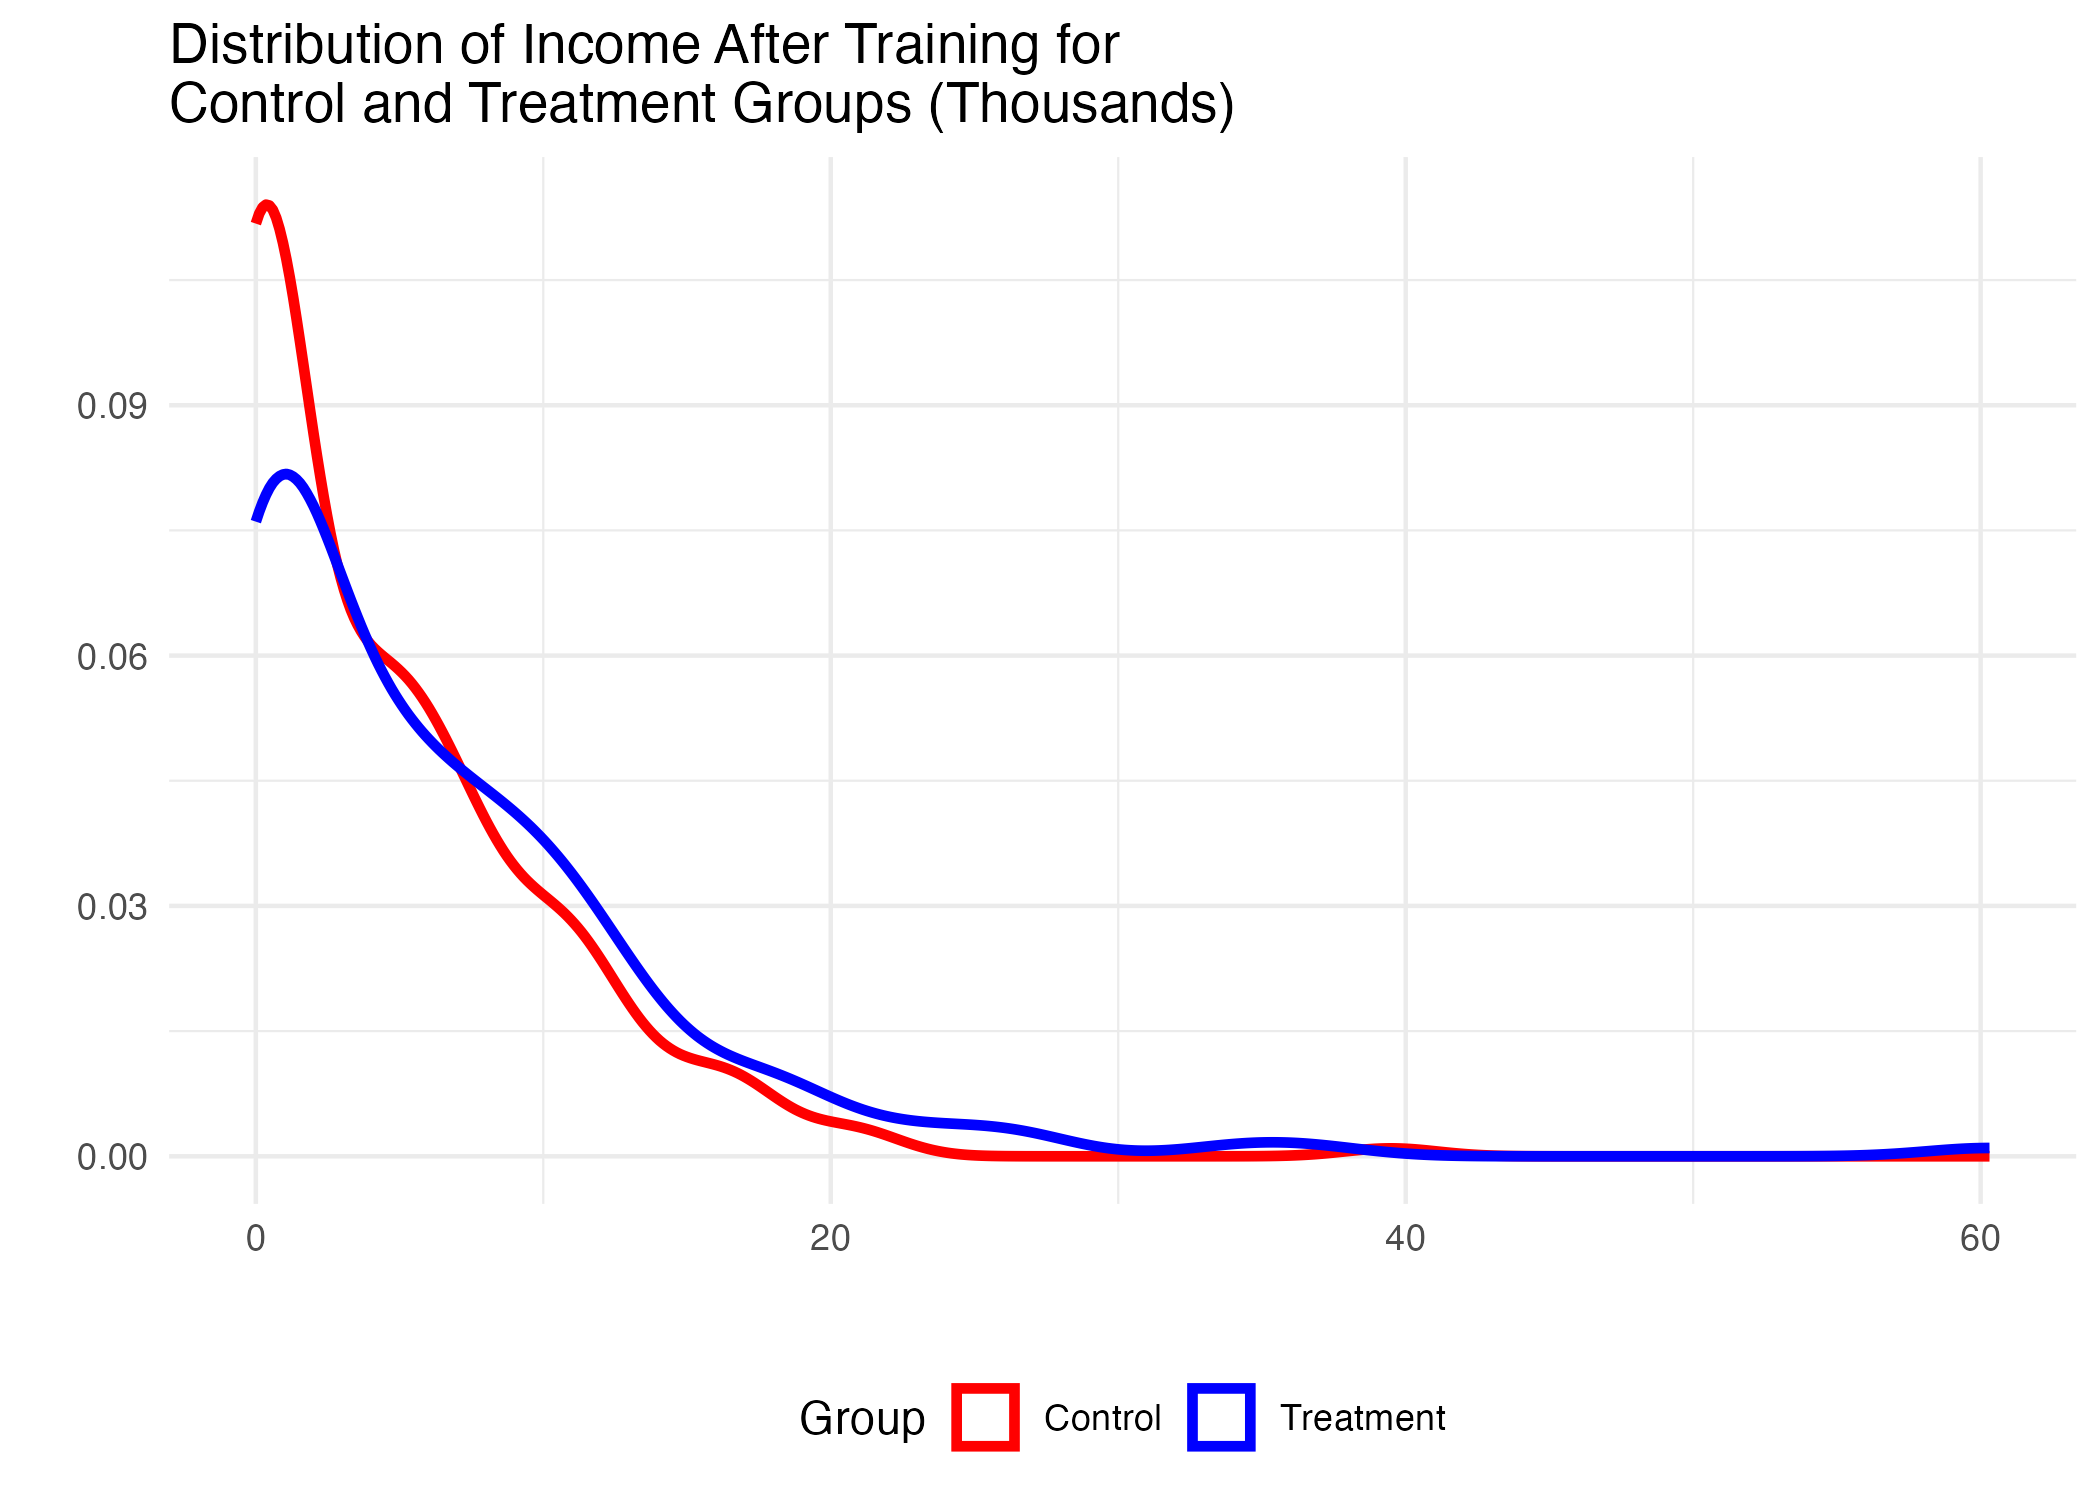
\includegraphics[width=\textwidth]{distribution_of_income_after_training_for_treatment_and_control.png}
    \caption{Distribution for Treatment and Control Groups}
    \label{fig:your_image_label}
\end{figure}

In this plot we see:
\begin{itemize}
    \item Overlap and Variability: the earning distributions for both groups show significant overlap, especially in the lower range of earnings. This overlap introduces uncertainty in interpreting the ATT as a straighforward policy impact.
    \item Skewness and Outliers: the treatment group has a long tail, showing that the ATT is influenced by the outliers. This highlights that the training might be highly beneficial for some individuals, but not beneficial for all.
    \item Variability of the ATT: the distribution highlights possibly the variability of the outcome. Therefore, it is strongly indicated to measure the variance of the ATT and look for targeted or conditional programs, aiming the training at only those who benefit from it. Policymakers should use the available features to investigate where the treatment is most useful.
\end{itemize}

The following table shows the deciles of the variable \texttt{income.after}.

Up until the percentile 30, the \texttt{income.after} $= 0$.

\begin{table}[H]
\centering
\begin{tabular}{|l|c|c|}
\hline
\textbf{Income Decile} & \textbf{Nº Control} & \textbf{Nº Treatment} \\
\hline
1D to 3D & 92 & 45 \\
4D       & 20 & 21 \\
5D       & 26 & 19 \\
6D       & 27 & 17 \\
7D       & 28 & 16 \\
8D       & 23 & 22 \\
9D       & 25 & 19 \\
10D      & 19 & 26 \\
\hline
\end{tabular}
\caption{Distribution of Earnings for Control and Treatment Groups by Income Group}
\label{tab:earnings_distribution}
\end{table}

By reducing the number of individuals in the lowest income quantiles and increasing those in the higher ones, the program demonstrates its potential to promote economic mobility. Nonetheless, the previous points again highlight the importance of researching further before providing policymaking conclusions.

\begin{colorparagraph}{questioncolor}
\label{q4c}\subsection{Statistical Uncertainty Around the ATT}
(c) We wish to assess the statistical uncertainty around the ATT estimate. Do this by (i) obtaining an influence function representation for the difference in means estimate, (ii) using this result to prove that the estimator is asymptotically normal and characterize the asymptotic variance, and (iii) propose consistent standard errors. Compute a 90\% confidence interval.

\rule{\textwidth}{0.5pt}
\end{colorparagraph}

\textbf{Influence Function Representation for the Difference in Means Estimate}

As we saw in the previous questions, in a randomized controlled trial, the Average Treatment Effect on the Treated (ATT) is estimated by the difference in sample means between the treatment and control groups:

\[
\hat{\tau}_{\text{ATT}} = \bar{Y}_1 - \bar{Y}_0
\]

Influence Function Derivation:

The influence function (IF) represents the impact of an individual observation on the estimator. For the difference in means estimator, the influence function is:

\[
\text{IF}_i = \frac{D_i}{p} (Y_i - \mu_1) - \frac{(1 - D_i)}{1 - p} (Y_i - \mu_0)
\]

where:

\begin{itemize}
    \item \(D_i\) is the treatment indicator (\(D_i = 1\) if treated, \(D_i = 0\) if control).
    \item \(p = P(D_i = 1)\) is the probability of receiving treatment.
    \item \(\mu_1 = E[Y_i | D_i = 1]\) is the population mean outcome for the treated.
    \item \(\mu_0 = E[Y_i | D_i = 0]\) is the population mean outcome for the control.
\end{itemize}

This influence function captures the deviation of each individual's outcome from the group mean, scaled by the probability of treatment assignment.

\textbf{Asymptotic Normality and Asymptotic Variance}

Under standard regularity conditions (e.g., independent and identically distributed samples, finite variances), the difference in sample means is asymptotically normally distributed:

\[
\sqrt{n} (\hat{\tau}_{\text{ATT}} - \tau_{\text{ATT}}) \xrightarrow{d} \mathcal{N}(0, \sigma^2)
\]

where:

\begin{itemize}
    \item \(n\) is the total sample size.
    \item \(\tau_{\text{ATT}} = \mu_1 - \mu_0\) is the true ATT.
    \item \(\sigma^2\) is the asymptotic variance of the estimator.
\end{itemize}

The asymptotic variance is derived from the variance of the influence function:

\[
\sigma^2 = E[\text{IF}_i^2] = \frac{\sigma_1^2}{p} + \frac{\sigma_0^2}{1 - p}
\]

where:

\begin{itemize}
    \item \(\sigma_1^2 = \text{Var}(Y_i | D_i = 1)\) is the variance of outcomes in the treatment group.
    \item \(\sigma_0^2 = \text{Var}(Y_i | D_i = 0)\) is the variance of outcomes in the control group.
\end{itemize}

This expression reflects that the variance of the estimator depends on the variability within each group and the proportion of the sample in each group.

\textbf{Consistent Standard Errors and 90\% Confidence Interval}

Estimating Variances and Standard Error:

Using the sample data, we calculate:

\begin{itemize}
    \item Sample Sizes:
        \begin{itemize}
            \item \(n_1 =\) Number of treated individuals.
            \item \(n_0 =\) Number of control individuals.
        \end{itemize}
    \item Sample Means:
        \begin{itemize}
            \item \(\bar{Y}_1 =\) Mean income after training for the treated group.
            \item \(\bar{Y}_0 =\) Mean income after training for the control group.
        \end{itemize}
    \item Sample Variances:
        \begin{itemize}
            \item \(s_1^2 =\) Sample variance in the treated group.
            \item \(s_0^2 =\) Sample variance in the control group.
        \end{itemize}
\end{itemize}

Given Results:

\begin{itemize}
    \item Estimated ATT:
        \[
        \hat{\tau}_{\text{ATT}} = \bar{Y}_1 - \bar{Y}_0 = \$1,794.34
        \]
    \item Standard Error:
        \[
        \text{SE}(\hat{\tau}_{\text{ATT}}) = \$670.997
        \]
    \item 90\% Confidence Interval:
        \[
        \text{CI}_{90\%} = [\$690.65, \$2,898.03]
        \]
\end{itemize}

Standard Error Calculation:

\[
\text{SE}(\hat{\tau}_{\text{ATT}}) = \sqrt{\frac{s_1^2}{n_1} + \frac{s_0^2}{n_0}}
\]

The standard error combines the variability of both groups, adjusted for their sample sizes.

Confidence Interval Calculation:
For a 90\% confidence interval, the critical value \(z_{\alpha/2}\) corresponds to the 95th percentile of the standard normal distribution (\(\alpha = 0.10\), two-tailed test).

\[
z_{\alpha/2} = 1.645
\]

Lower Bound:
\[
\text{Lower} = \hat{\tau}_{\text{ATT}} - z_{\alpha/2} \times \text{SE}(\hat{\tau}_{\text{ATT}}) = 1,794.34 - 1.645 \times 670.997 = \$690.65
\]

Upper Bound:
\[
\text{Upper} = \hat{\tau}_{\text{ATT}} + z_{\alpha/2} \times \text{SE}(\hat{\tau}_{\text{ATT}}) = 1,794.34 + 1.645 \times 670.997 = \$2,898.03
\]

Interpretation:

\begin{itemize}
    \item Estimated ATT (\$1,794.34): On average, participants who received job training earned \$1,794.34 more than those who did not.
    \item 90\% Confidence Interval (\$690.65 to \$2,898.03): The entire interval is above zero, indicating a statistically significant positive effect at the 10\% significance level. Since the confidence interval does not include zero, the effect of job training is statistically significant.
\end{itemize}

Policymakers can be reasonably assured of the program's beneficial impact, with expected earnings increases ranging from approximately \$690 to \$2,898.

Given the positive impact, it may be advisable to continue or expand the program. Further investigations of covariates should be useful to decide if the program should target the entire population or subsets of it.

\begin{figure}[H]
\centering
\begin{lstlisting}[style=Rstyle, caption=90\% Confidence Interval]
n1 <- sum(nsw_rct$treat == 1)
n0 <- sum(nsw_rct$treat == 0)
n <- n1 + n0

mean_treated <- mean(nsw_rct$income.after[nsw_rct$treat == 1])
mean_control <- mean(nsw_rct$income.after[nsw_rct$treat == 0])

var_treated <- var(nsw_rct$income.after[nsw_rct$treat == 1])
var_control <- var(nsw_rct$income.after[nsw_rct$treat == 0])

variance_att <- var_treated / n1 + var_control / n0

se_att <- sqrt(variance_att)

z_alpha <- qnorm(0.95)

lower_bound <- (mean_treated - mean_control) - z_alpha * SE_ATT
upper_bound <- (mean_treated - mean_control) + z_alpha * SE_ATT

cat("Estimated ATT:", mean_treated - mean_control, "\n")
# Estimated ATT: 1794.342 

cat("Standard Error:", se_att, "\n")
# Standard Error: 670.9965

cat("90% Confidence Interval: [", lower_bound, ",", upper_bound, "]\n")
# 90% Confidence Interval: [ 690.6513 , 2898.034 ]
\end{lstlisting}
\end{figure}

\begin{colorparagraph}{questioncolor}
\label{q4d}\subsection{Maximizing Welfare Through Targeting Rules}
(d) We want to maximize welfare using targeting rules. To make the resulting policy easy to implement and transparent, it must be a threshold policy based on a single covariate, so search for rules of the form \( d(x) = 1\{x_j > c\} \) or \( d(x) = 1\{x_j < c\} \) for a specific covariate \( x_j \) and some cutoff value \( c \). What is the welfare maximizing rule?

\rule{\textwidth}{0.5pt}
\end{colorparagraph}

We consider the welfare maximimizing rule the rule that generates the biggest total income (sum of the entire sample \texttt{income.after}). In other words, we aim to find the $d(x)$ that solves the following:

$$
\max_{d(x)} \sum_{i = 1}^{n} \text{income.after}_i(d(x))
$$

Where $\text{income.after}_i(d(x))$ is the potential outcome for $t_i = d(x)$.

Therefore, we aim for $d(x)$ that:
\begin{itemize}
    \item Contains a big group
    \item Contains an above average CATE.
\end{itemize}

In total, the welfare will be computed as:

$$
\text{CATT}_i = \mathbb{E}[Y_i | t_i = 1, d_i = 1] - \mathbb{E}[Y_i | t_i = 0, d_i = 1]
$$

$$
\Delta \text{Welfare} = \text{CATT} \times \sum_{i = 1}^{n} d_i
$$

Meaning, the bigger the number of observations in $d_i = 1$, the bigger the welfare generated. The bigger the CATT, the bigger the welfare generated.

We run an optimization in both the binary and continuous variables. In the binary variables, we check both options. In the continuous variables, we check the threshold for every single sample variable.

\begin{figure}[H]
\centering
\begin{lstlisting}[style=Rstyle, caption=Binary Threshold Search]
binary_covariate_list <- c("black", "hispanic", "married", "hsdegree")

all_binary_groups_att <- data.frame()

for (binary_covariate in binary_covariate_list) {
  group_att <- nsw_rct %>%
    rename(covariate := !!binary_covariate) %>% 
    group_by(treat, covariate) %>% 
    summarise(
      avg = mean(income.after)
    ) %>% 
    ungroup() %>% 
    spread(treat, avg) %>% 
    purrr::set_names("covariate", "control_mean", "treatment_mean") %>% 
    mutate(att_group = treatment_mean - control_mean) %>% 
    left_join(
      nsw_rct %>% 
        rename(covariate := !!binary_covariate) %>% 
        group_by(covariate) %>% 
        summarise(
          n = n()
        ) %>% 
        ungroup()
    ) %>% 
    mutate(wealth = n * att_group) %>% 
    mutate(covariate_name = binary_covariate)
  all_binary_groups_att <- all_binary_groups_att %>% rbind(group_att)
}

all_binary_groups_att <- all_binary_groups_att %>% 
  mutate(covariate_threshold = paste(covariate_name, "=", covariate))

\end{lstlisting}
\end{figure}

\begin{figure}[H]
\centering
\begin{lstlisting}[style=Rstyle, caption=Continous Variables Threshold Search]
discrete_covariate_list <- c("age", "education", "income.before1", "income.before2")

all_discrete_groups_att <- data.frame()

for (discrete_covariate in discrete_covariate_list) {
  
  covariate_unique_values <- nsw_rct %>%
    rename(covariate := !!discrete_covariate) %>%
    arrange(covariate) %>% 
    .$covariate %>% unique()
  
  for (covariate_value in covariate_unique_values) {
    
    new_covariate_name <- paste(discrete_covariate, "<=", covariate_value)
    
    group_att <- nsw_rct %>%
      rename(covariate := !!discrete_covariate) %>% 
      mutate(covariate = ifelse(covariate <= covariate_value, 1, 0)) %>% 
      group_by(treat, covariate) %>% 
      summarise(
        avg = mean(income.after)
      ) %>% 
      ungroup() %>% 
      spread(treat, avg) %>% 
      purrr::set_names("covariate", "control_mean", "treatment_mean") %>% 
      mutate(att_group = treatment_mean - control_mean) %>% 
      left_join(
        nsw_rct %>% 
          rename(covariate := !!discrete_covariate) %>% 
          mutate(covariate = ifelse(covariate <= covariate_value, 1, 0)) %>% 
          group_by(covariate) %>% 
          summarise(
            n = n()
          ) %>% 
          ungroup()
      ) %>% 
      mutate(wealth = n * att_group) %>% 
      mutate(covariate_name = discrete_covariate) %>% 
      mutate(covariate_threshold = ifelse(covariate == 0, sub("<=", ">", new_covariate_name), new_covariate_name))
    all_discrete_groups_att <- all_discrete_groups_att %>% rbind(group_att)
  }
}
\end{lstlisting}
\end{figure}

\begin{table}[H]
    \centering
    \begin{tabular}{|c|c|c|c|c|c|}
    \hline
    \textbf{Rule} & \textbf{Avg Control} & \textbf{Avg Treatment} & \textbf{CATT} &
    \textbf{Nº} & \textbf{Welfare} \\
    \hline
    $\text{income.before1} \leq 2143.413$ & 4116.11 & 6644.19 & 2528.07 & 355 & 897467.37 \\
    $\text{income.before1} \leq 2192.877$ & 4116.11 & 6622.40 & 2506.28 & 356 & 892237.49 \\
    $\text{income.before1} \leq 492.2305$ & 4028.62 & 6741.84 & 2713.21 & 328 & 889934.82 \\
    $\text{income.before1} \leq 2636.353$ & 4112.97 & 6567.47 & 2454.50 & 361 & 886074.68 \\
    $\text{income.before1} \leq 2431.949$ & 4096.61 & 6560.92 & 2464.31 & 359 & 884690.31 \\
    \hline
    \end{tabular}
    \caption{Best Simple Rules to Maximize Welfare}
    \label{tab:earnings_distribution}
\end{table}

\begin{table}[H]
    \centering
    \begin{tabular}{|c|c|c|c|c|c|}
    \hline
    \textbf{Rule} & \textbf{Avg Control} & \textbf{Avg Treatment} & \textbf{CATT} &
    \textbf{Nº} & \textbf{Welfare}$^{*}$ \\
    \hline
    $\text{income.before1} \leq 2143.413$ & 4116.11 & 6644.19 & 2528.07 & 355 & 897467.4 \\
    $\text{age} \leq 42$                  & 4479.29 & 6492.98 & 2013.68 & 429 & 863872.5 \\
    $\text{income.before2} \leq 13830.64$ & 4492.43 & 6374.98 & 1882.55 & 440 & 828324.7 \\
    $\text{education} \geq 8$             & 4662.35 & 6833.28 & 2170.92 & 381 & 827123.7 \\
    $\text{hispanic} = 0$                 & 4340.58 & 6300.25 & 1959.66 & 406 & 795623.1 \\
    $\text{black} = 1$                    & 4107.65 & 6136.32 & 2028.66 & 371 & 752636.2 \\
    $\text{married} = 0$                  & 4646.50 & 6019.99 & 1373.49 & 370 & 508192.6 \\
    $\text{hsdegree} = 0$                 & 4495.41 & 5649.46 & 1154.04 & 348 & 401608.4 \\
    \hline
    \end{tabular}
    \caption{Best Simple Rules to Maximize Welfare for each Covariate}
    \label{tab:earnings_distribution}
\end{table}

*Welfare increase generate by the training: $\text{CATT} \times \text{Nº}$

\begin{figure}[H]
    \centering
    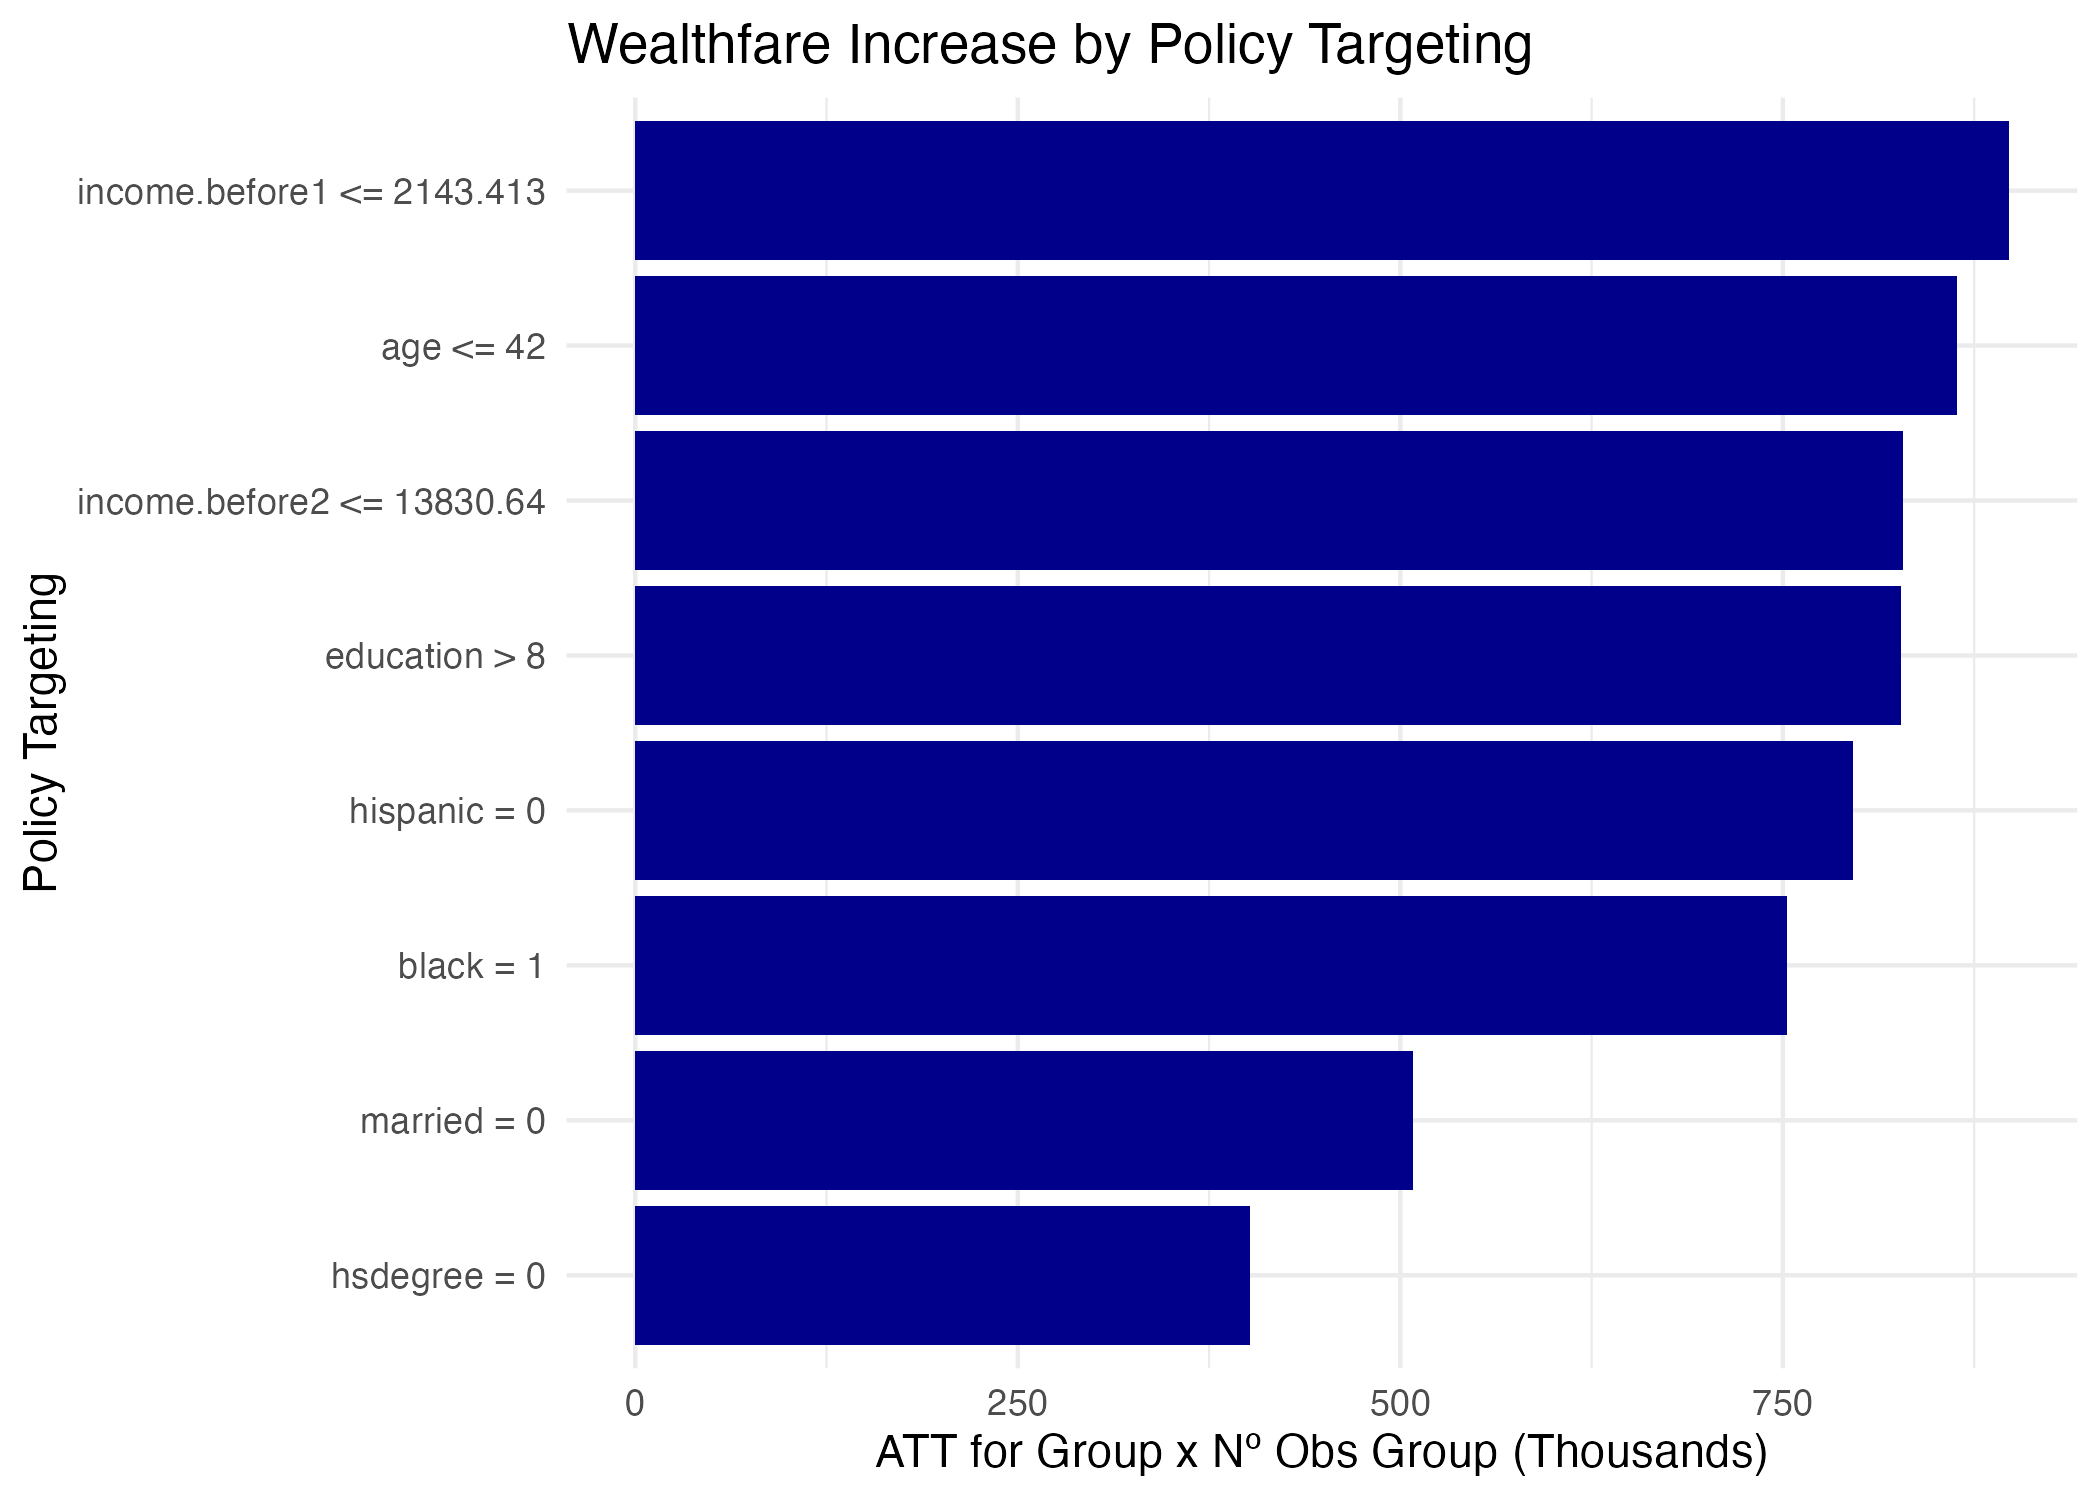
\includegraphics[width=\textwidth]{wealth_increase_by_policy_targeting.png}
    \caption{Best Simple Rules to Maximize Welfare for each Covariate}
    \label{fig:your_image_label}
\end{figure}

Thus, the best rule found is $d = \mathbb{I} \{ \text{income.before1} \leq 2143.413\}$. Meaning that the treatment should only be applied to people with income in the previous year less or equal to \$2,1 thousands.

This highlight that it is better to apply the training to only a subset of the population than to the entire sample.

This happens because the CATT of the group is considerably larger than the ATT to compensate for the decrease in number of target units.

$$
\begin{aligned}
    \text{ATT} \times n &< \text{CATT} \times n_{\text{target}} \\
    1794.342 \times 445 &< 2528.07 \times 355 \\
    798482.2 &< 897467.4
\end{aligned}
$$

\begin{colorparagraph}{questioncolor}
\rule{\textwidth}{0.5pt}

\label{q4e}\subsection{Role of Group Size in Targeting}
(e) What role does the size of the group flagged by \( d(x) \) play in your conclusions?

\rule{\textwidth}{0.5pt}
\end{colorparagraph}

The formula defined for welfare increase by training:

$$
\Delta \text{Welfare} = \sum_{i = 1}^{n} d_i \text{CATT}_i
$$

Since the $\text{CATT}_i$ matches for all in the target:

$$
\Delta \text{Welfare} = \text{CATT} \sum_{i = 1}^{n} d_i
$$


Welfare increase is a multiplication of the CATT for the group which should receive training by the amount of people who should receive training ($\sum_{i = 1}^{n} d_i$).

Meaning, $\sum_{i = 1}^{n} d_i$ is the size of the group flagged (also called $n_{\text{target}}$).

In other words, for groups that have bigger $\text{CATT}$ but are less representative in the population, the expected welfare generated is smaller.

For instance:

\begin{itemize}
    \item The $d = \mathbb{I} \{ \text{income.before1} > 33799.95 \}$ provide ATT for the targeted group of 33563.369. Nonetheless, the amount of people in the sample is 2 ($< 1\%$ of sample).
    \item The $d = \mathbb{I} \{ \text{education} > 12 \}$ provides ATT for the treated group 7149.948. Nonetheless, $n_{\text{target}} = 22$ for the treated group in the sample ($5\%$ of sample).
    \item The $d = \mathbb{I} \{ \text{married} = 1 \}$ provides ATT for the treated group 3709.335. Nonetheless, $n_{\text{target}} = 75$ for the treated group in the sample ($17\%$ of sample).
\end{itemize}

The optimal strategy provides ATT of 2528.077 for the treated group, smaller than the previous examples, nonetheless, it contains $n_{\text{target}} = 355$ ($80\%$ of sample).

The solution highlights the importance of having a sample with characteristics representative of the entire population. We expect that $d = \mathbb{I} \{ \text{income.before1} \leq 2143.413 \}$ represents 80\% of the population as well.

\newpage

\begin{colorparagraph}{questioncolor}
\rule{\textwidth}{0.5pt}

\label{q4f}\subsection{Testing Targeting Rules for Welfare Improvement}
(f) Explain how you would statistically test the effectiveness of your targeting rule on improving welfare.

\rule{\textwidth}{0.5pt}
\end{colorparagraph}

For this question, we do the test with two different methodologies, as discussed during the TA Office Hours.

Those are:
\begin{itemize}
    \item Difference for ATT of target group (inside our policy) and ATT of non-target group (outside our policy).
    \item Significance of the ATT for the target group (group inside our policy).
\end{itemize}

\textbf{Difference in ATT for Target and Non-Target Group}

To test the effectiveness of our solution, check if there is a significant difference in ATT of the target group and the ATT of the non-target group.

$$
H_0 : \text{CATT}_{\text{target}} \leq \text{CATT}_{\text{non-target}} 
$$

$$
H_a : \text{CATT}_{\text{target}} > \text{CATT}_{\text{non-target}} 
$$

Again:

\begin{itemize}
    \item Target Group: Individuals with income.before1 $\leq 2143.413$, to whom we plan to apply the treatment under your new policy.
    \item Non-Target Group: Individuals with income.before1 $> 2143.413$, to whom we will not apply the treatment.
\end{itemize}

We can more easily test that with a regression:

$$
\text{income.after}_i = \beta_0 + \beta_1 \times \text{treat}_i + \beta_2 \times \text{target}_i + \beta_3 \times \text{treat}_i \times \text{target}_i + \varepsilon
$$

\begin{figure}[H]
\centering
\begin{lstlisting}[style=Rstyle, caption=ATT]
lm(
  income.after ~ target * treat + treat + target,
  data=nsw_rct %>% 
    mutate(target = ifelse(income.before1 <= 2143.413, 1, 0))
) %>% summary()

"""
Call:
lm(formula = income.after ~ target * treat + treat + target, 
    data = nsw_rct %>% mutate(target = ifelse(income.before1 <= 
        2143.413, 1, 0)))

Residuals:
   Min     1Q Median     3Q    Max 
 -6644  -4116  -1702   3168  53664 

Coefficients:
             Estimate Std. Error t value Pr(>|t|)    
(Intercept)      6397        926   6.908 1.72e-11 ***
target          -2281       1030  -2.214   0.0274 *  
treat           -1118       1389  -0.805   0.4215    
target:treat     3646       1559   2.339   0.0198 *  
---
Signif. codes:  0 '***' 0.001 '**' 0.01 '*' 0.05 '.' 0.1 ' ' 1

Residual standard error: 6548 on 441 degrees of freedom
Multiple R-squared:  0.03158,	Adjusted R-squared:  0.02499 
F-statistic: 4.793 on 3 and 441 DF,  p-value: 0.002688
"""
\end{lstlisting}
\end{figure}

The results in the data translate to:

$$
\hat{\text{income.after}}_i = 6397 - 1118 \times \text{treat}_i - 2281 \times \text{target}_i + 3646 \times \text{treat}_i \times \text{target}_i
$$

In the regression:
\begin{itemize}
    \item $\hat{\beta}_0 = 6397$ is the average income.after for the non-target group.
    \item $\hat{\beta}_0 + \hat{\beta}_1 = 6397 - 2281$ is the average income.after for the target group.
    \item $\hat{\beta}_2 = -1118$ is the treatment effect for the non-target group.
    \item $\hat{\beta}_2 + \hat{\beta}_3 = -1118 + 3646$ is the treatment effect for the target group. 
\end{itemize}

$\hat{\beta}_3$ is significant at 5\%, meaning that the ATT for the target group is significantly different from the ATT of the non-target group.

\textbf{Significance of ATT for Target Group}

To test the effectiveness of the target rule in improving welfare, we determine whether or not the observed increase in welfare under the targeting rule is statistically significant.

$$
H_0 : \text{CATT}_{\text{target}} \leq 0
$$

$$
H_a : \text{CATT}_{\text{target}} > 0
$$

Where the $\text{CATT}$ is the ATT only for the target group of the policy. In our example, the target group of our policy is $\text{income.before}_i \leq 2143.413$. Thus, we only use the sub group of the sample where the condition hold and check the significance of the training in it.

\begin{figure}[H]
\centering
\begin{lstlisting}[style=Rstyle, caption=Test of Difference in Means]
nws_rct_filtered_target_rule <- nsw_rct %>% 
  filter(income.before1 <= 2143.413) %>% 
  mutate(reverse_treat = 1 - treat)

t.test(
    income.after ~ treat,
    data = nws_rct_filtered_target_rule,
    alternative = "less", var.equal = FALSE
)

"""
Welch Two Sample t-test

data:  income.after by treat
t = -3.3688, df = 211.29, p-value = 0.0004486
alternative hypothesis: true difference in means between group 0 and group 1 is less than 0
95 percent confidence interval:
      -Inf -1288.286
sample estimates:
mean in group 0 mean in group 1 
       4116.118        6644.195 
"""

# Which is equal to:

t.test(
    income.after ~ reverse_treat,
    data = nws_rct_filtered_target_rule,
    alternative = "greater", var.equal = FALSE
)

"""
Welch Two Sample t-test

data:  income.after by reverse_treat
t = 3.3688, df = 211.29, p-value = 0.0004486
alternative hypothesis: true difference in means between group 0 and group 1 is greater than 0
95 percent confidence interval:
 1288.286      Inf
sample estimates:
mean in group 0 mean in group 1 
       6644.195        4116.118 
"""
\end{lstlisting}
\end{figure}

We arrive to a significant difference in mean for the two methods, generating the conclusion that there is a positive ATT for the specified target group.

\begin{colorparagraph}{questioncolor}
\rule{\textwidth}{0.5pt}

\label{q4g}\subsection{Demographic Characteristics of Targeted Individuals}
(g) Examine the demographic characteristics of who your program targets compared to who is not targeted. What do you find and is this pattern concerning? (\textit{A real study should compare the targeted demographics to the relevant/eligible population, e.g., the whole city.})

\rule{\textwidth}{0.5pt}
\end{colorparagraph}

\begin{figure}[H]
\centering
\begin{lstlisting}[style=Rstyle, caption=Data Statistics Code]
nsw_rct %>% 
  mutate(target = ifelse(income.before1 <= 2143.413, 1, 0)) %>% 
  group_by(target) %>% 
  summarise(
    avg_income_after = mean(income.after),
    std_income_after = sd(income.after),
    pct_black = mean(black),
    pct_married = mean(married),
    pct_hispanic = mean(hispanic),
    pct_treated = mean(treat),
    avg_education = mean(education),
    std_education = sd(education),
    avg_age = mean(age, na.rm = TRUE),
    std_age = sd(age, na.rm = TRUE),
    n = n(),
    avg_income_before2 = mean(income.before2),
    std_income_before2 = sd(income.before2),
    avg_income_before1 = mean(income.before1),
    std_income_before1 = sd(income.before1),
  ) %>% 
  gather(id, value, -target) %>% 
  spread(target, value) %>% 
  mutate(id = factor(id, levels = covariate_levels)) %>% 
  arrange(id)
\end{lstlisting}
\end{figure}

\begin{table}[H]
    \centering
    \begin{tabular}{|l|c|c|}
    \hline
    \textbf{Covariate} & \textbf{Non-Target} & \textbf{Target} \\
    \hline
    Avg. Income After (Y)  & 5901 & 5149 \\   
    Std. Income After (Y)  & 7284 & 6458 \\  
    \% Treated             & 44.4\% & 40.8\% \\ 
    \% Black               & 80\%   & 84.2\% \\ 
    \% Married             & 23.3\% & 15.2\% \\ 
    \% Hispanic            & 10\%   & 8.54\% \\
    \% HSDegree            & 27.8\%   & 20.3\% \\
    Avg. Education         & 10.5  & 10.1 \\   
    Std. Education         & 1.61  & 1.83 \\  
    Avg. Age               & 25.1  & 25.4 \\   
    Std. Age               & 5.83  & 7.39 \\  
    N. Obs                 & 90    & 355 \\
    Avg. Income Before 1   & 10007 & 98.3 \\   
    Std. Income Before 1   & 7988 & 359 \\  
    Avg. Income Before 2   & 4967 & 467 \\   
    Std. Income Before 2   & 5017 & 1420 \\  
    \hline
    \end{tabular}
    \caption{Statistics Covariates in Target and Non-Target Groups}
    \label{tab:earnings_distribution}
\end{table}

The differences in covariates between target and non-target group are:
\begin{itemize}
    \item Average \texttt{income.before1} and \texttt{income.before2} are considerably lower for the target group.
    \item The non-target has more married people (50\% more than target).
    \item Hispanics are under represented in the target population. The oppositve happens for black.
    \item The percentage of subjects who completed high school is 7 p.p. higher in the non-target group.
\end{itemize}

The reliance on prior income as the sole criterion may lead to unintentional bias. In some cases, the bias can be viewed as prejudice. For instance, hispanics or married individuals might feel under represented in the program.

On the other hand, leading a program with such target rule might be easier to advertise, since it only explicitly aims to target people in worst social condition. In this sense, this could be viewed as program targeting equality (while actually bigger equality of outcome would be a consequence).

Happily, the differences in covariates are not monumental between target and non-target groups and, for many of the these, the average and standard deviation are approximately the same. Therefore, while we should be concerned about correctly advertising such program, the differences in statistics between non-target and target group are not extremely concerning.

\begin{colorparagraph}{questioncolor}
\rule{\textwidth}{0.5pt}

\label{q42}\subsection*{Observational Data}

Suppose there was no experiment. We have data from the same 185 men that received job training but we do not have access to the NSW control sample. For a comparison sample we found 2490 men from the Panel Study of Income Dynamics (PSID) that did not have training. The data is in \texttt{nsw\_PSID.csv}.

\rule{\textwidth}{0.5pt}
\end{colorparagraph}

\begin{colorparagraph}{questioncolor}
\label{q4h}\subsection{Concerns with Observational Data}
(h) Before beginning the analysis, summarize the main concern when it comes to using observational data for the analysis. Why might the PSID \textit{comparison} group not be a good control group?

\rule{\textwidth}{0.5pt}
\end{colorparagraph}

The main concern relates to selection bias, meaning that, unlike randomized controlled trials (RCTs), where the randomization ensures that treatment and control groups are statistically equivalent on both observed and unobserved characteristics (in expectation), observational studies lack this safeguard. 

More specifically:
\begin{itemize}
    \item Selection on unobserved: individuals self-select into treatment based on characteristics that may notbe observed or measured by data (e.g. motivation, employment history, social networks, ambition). If the unobserved factors correlated with the likelihood of receiving treatment and the outcome variable (income after), the estimate of treatment effect should be biased .
    \item Demographic covariates of treatment and control: the treated and control groups may differ systematically in observable characteristics. Failing to account for them when estimating the effect of the treatment may result in biased estimates.
    \item Uncertainty if assignment of treatment is independent of potential outcome: in randomized trials, we can say that the the potential outcome is orthogonal to the assignment. In observable data, we hope that the potential outcome is orthoginal to the assignment conditional on the covariates. In other words, meaning that the covariates are able to fix this issue. Nonetheless, we cannot affirm the latter holds and, if not, even the ATE conditioning on covariates is biased.
\end{itemize}

\begin{colorparagraph}{questioncolor}
\rule{\textwidth}{0.5pt}    

\label{q4i}\subsection{Estimation Using PSID Control Sample}
(i) Using the PSID control sample as though it were the control group for a randomized trial, estimate the average treatment effect. Explain what you find and why you found it.

\rule{\textwidth}{0.5pt}
\end{colorparagraph}

\begin{figure}[H]
\centering
\begin{lstlisting}[style=Rstyle, caption=ATT for Observational Data]
nsw_psid %>% 
  group_by(treat) %>% 
  summarise(avg = mean(income.after)) %>% 
  spread(treat, avg) %>% 
  purrr::set_names(c("control", "treatment")) %>% 
  mutate(att = treatment - control)

"""
  # A tibble: 1 x 3
  control treatment     att
    <dbl>     <dbl>   <dbl>
1  21554.     6349. -15205.
"""
\end{lstlisting}
\end{figure}

The estimated ATE is -\$15,205. This suggests that participating in the job training program is associated with an average decrease in earnings of \$15,205 compared to the control group. In other words, the estimate implies that the job training program had a large negative effect on earnings.

This result is counterintuitive, as we would typically expect job training to have a positive impact on earnings. The negative estimated effect arises due to significant differences between the treatment and control groups, leading to biased estimates. 

Among the difference in covariates between the treatment and control groups, we find:
\begin{itemize}
    \item Avg Income 1 Year Before:
    \begin{itemize}
        \item Treatment Group: \$2,096
        \item Control Group: \$19,429
    \end{itemize}
    \item Avg Income 2 Year Before:
    \begin{itemize}
        \item Treatment Group: \$1,532
        \item Control Group: \$19,063
    \end{itemize}
\end{itemize}

The control group had substantially higher earnings before the treatment period. This indicates that they were economically better off even before the job training program was introduced. In other words, The treatment group consisted of economically disadvantaged individuals.

The assumption that treatment assignment is independent of potential outcomes does not hold in this observational setting. The lack of randomization means that the differences in outcomes may be due to pre-existing differences rather than the effect of the job training program.

Therefore, the negative estimate is a result of confounding factors that are not accounted for when simply comparing the means. By treating the PSID control sample as if it were from a randomized trial, we ignore the significant differences in baseline characteristics. This leads to an estimate that reflects the pre-existing disparities rather than the effect of the job training program.

In conclusion, we should state that the ATE of -\$15,205 is not a credible estimate of the causal effect of the job training program.

\newpage

\begin{colorparagraph}{questioncolor}
\rule{\textwidth}{0.5pt}

\label{q4j}\subsection{Suitability of the PSID as a Control Group}
(j) Does the PSID sample appear to be a good control group for this purpose? That is, using the covariates, does the treatment appear to be randomly assigned?

\rule{\textwidth}{0.5pt}
\end{colorparagraph}

\begin{figure}[H]
\centering
\begin{lstlisting}[style=Rstyle, caption=Data Statistics Code]
nsw_psid %>% 
  group_by(treat) %>% 
  summarise(
    avg_income_after = mean(income.after),
    std_income_after = sd(income.after),
    pct_black = mean(black),
    pct_married = mean(married),
    pct_hispanic = mean(hispanic),
    avg_education = mean(education),
    std_education = sd(education),
    avg_age = mean(age, na.rm = TRUE),
    std_age = sd(age, na.rm = TRUE),
    n = n(),
    avg_income_before2 = mean(income.before2),
    std_income_before2 = sd(income.before2),
    avg_income_before1 = mean(income.before1),
    std_income_before1 = sd(income.before1),
  ) %>% 
  gather(id, value, -treat) %>% 
  spread(treat, value) %>% 
  mutate(id = factor(id, levels = covariate_levels)) %>% 
  arrange(id)
\end{lstlisting}
\end{figure}

\begin{table}[H]
    \centering
    \begin{tabular}{|l|c|c|}
    \hline
    \textbf{Covariate} & \textbf{Control} & \textbf{Treatment} \\
    \hline
    Avg. Income After (Y)  & 21554     & 6349 \\
    Std. Income After (Y)  & 15555     & 7867 \\
    \% Black               & 25.1\%     & 84.3\% \\
    \% Married             & 86.6\%     & 18.9\% \\
    \% Hispanic            & 3.25\%    & 5.95\% \\
    \% HSDegree            & 69.5\%    & 29.2\% \\
    Avg. Education         & 12.1      & 10.3 \\
    Std. Education         & 3.08      & 2.01 \\
    Avg. Age               & 34.9      & 25.8 \\
    Std. Age               & 10.4      & 7.16 \\
    N. Obs                 & 2490      & 185 \\
    Avg. Income Before 1   & 19429     & 2096 \\
    Std. Income Before 1   & 13407     & 4887 \\
    Avg. Income Before 2   & 19063     & 1532 \\
    Std. Income Before 2   & 13597     & 3219 \\
    \hline
    \end{tabular}
    \caption{Statistics Covariates in Treatment and Control Groups}
    \label{tab:earnings_distribution}
\end{table}

Based on the covariate statistics, the PSID sample does not appear to be a good control group for the NSW treatment group. There are substantial differences in observable characteristics between the two groups, indicating that the treatment assignment is not random when considering these covariates.

\begin{itemize}
    \item The control group had significantly higher earnings before the treatment period. The treatment group consists of individuals with very low pre-treatment earnings, indicating economic disadvantage. Such a large disparity suggests that the two groups are fundamentally different in terms of economic status prior to the intervention.
    \item The control group is more educated on average and has a higher proportion of individuals with at least a high school degree. Education level is a strong predictor of earnings.
    \item The control group is, on average, almost 9 years older than the treatment group. Age can significantly influence earnings potential and labor market experience.
    \item The treatment group has a much higher proportion of Black individuals. Racial disparities in labor markets can influence employment opportunities and earnings.
    \item A significantly higher proportion of the control group is married. Marital status can impact economic stability and household income.
    \item The control group continues to have higher earnings after the treatment period, likely reflecting pre-existing advantages rather than the effect of not receiving training.
\end{itemize}

Selection bias is clearly present in such experiment. The differences founds imply that the treatment group is systematically disadvantaged compared to the control group, and these disadvantages are correlated with both treatment assignment and the outcome (earnings).

The assumption that, conditional on observed covariates, treatment assignment is independent of potential outcomes (the ignorability or unconfoundedness assumption) does not hold.

\begin{colorparagraph}{questioncolor}
\rule{\textwidth}{0.5pt}

\label{q4k}\subsection{Controlling for Nonrandomization}
(k) Using the above to guide you, build a linear regression that attempts to control for any sources of nonrandomization. Does your regression-based treatment effect estimate recover the experimental benchmark treatment effect estimate? Discuss the uncertainty of your regression-based estimate and how this relates to the experimental benchmark.

\rule{\textwidth}{0.5pt}
\end{colorparagraph}

Running a regression with every covariate and the interaction of covariates with treatment provides a not interest result.

\begin{itemize}
    \item Most of the coefficients are not significant, due to the high multicollinearity of the regression.
    \item Treatment has a high negative impact (-\$2476).
    \item Income before 1 year and 2 years are the significant variables among the few variables with significant parameters, showcasing the importance of previous income to determine income after treatment.
\end{itemize}

\begin{figure}[H]
\centering
\begin{lstlisting}[style=Rstyle, caption=Model with Interactions]
Call:
lm(formula = income.after ~ ., data = nsw_psid_interaction_treat)

Residuals:
   Min     1Q Median     3Q    Max 
-65022  -4312   -420   3691 110204 

Coefficients:
                       Estimate Std. Error t value Pr(>|t|)    
(Intercept)           6.483e+02  1.447e+03   0.448   0.6542    
treat                -2.476e+03  6.480e+03  -0.382   0.7025    
age                  -9.357e+01  2.129e+01  -4.395 1.15e-05 ***
education             5.949e+02  1.060e+02   5.613 2.19e-08 ***
black                -5.707e+02  5.075e+02  -1.125   0.2609    
hispanic              2.503e+03  1.154e+03   2.169   0.0302 *  
married               1.381e+03  6.145e+02   2.247   0.0247 *  
income.before1        2.852e-01  2.819e-02  10.114  < 2e-16 ***
income.before2        5.675e-01  2.774e-02  20.455  < 2e-16 ***
hsdegree             -7.685e+02  6.786e+02  -1.133   0.2575    
income_before1_treat -2.457e-01  2.067e-01  -1.188   0.2348    
income_before2_treat -4.788e-01  3.137e-01  -1.526   0.1271    
black_treat          -5.693e+02  2.592e+03  -0.220   0.8261    
age_treat             1.771e+02  1.116e+02   1.587   0.1125    
married_treat        -3.483e+02  2.130e+03  -0.164   0.8701    
hispanic_treat       -2.198e+03  4.089e+03  -0.538   0.5909    
education_treat       2.910e+01  5.180e+02   0.056   0.9552    
hsdegree_treat        1.088e+03  2.416e+03   0.450   0.6526    
---
Signif. codes:  0 '***' 0.001 '**' 0.01 '*' 0.05 '.' 0.1 ' ' 1

Residual standard error: 10060 on 2657 degrees of freedom
Multiple R-squared:  0.5887,	Adjusted R-squared:  0.586 
F-statistic: 223.7 on 17 and 2657 DF,  p-value: < 2.2e-16
\end{lstlisting}
\end{figure}

When we run the regression without interactions, the treatment has positive coefficient. Nonetheless, its significance is still quite low.

\begin{lstlisting}[style=Rstyle, caption=Model without Interactions]
Call:
lm(formula = income.after ~ treat + age + education + black + 
    hispanic + married + hsdegree + income.before1 + income.before2, 
    data = nsw_psid)

Residuals:
   Min     1Q Median     3Q    Max 
-64870  -4302   -435   3786 110412 

Coefficients:
                 Estimate Std. Error t value Pr(>|t|)    
(Intercept)     460.72418 1408.89982   0.327   0.7437    
treat           751.94643  915.25723   0.822   0.4114    
age             -83.56559   20.81380  -4.015 6.11e-05 ***
education       592.61020  103.30278   5.737 1.07e-08 ***
black          -570.92797  495.17772  -1.153   0.2490    
hispanic       2163.28118 1092.29036   1.981   0.0478 *  
married        1240.51952  586.25391   2.116   0.0344 *  
hsdegree       -590.46695  646.78417  -0.913   0.3614    
income.before1    0.27812    0.02792   9.960  < 2e-16 ***
income.before2    0.56809    0.02756  20.613  < 2e-16 ***
---
Signif. codes:  0 '***' 0.001 '**' 0.01 '*' 0.05 '.' 0.1 ' ' 1

Residual standard error: 10070 on 2665 degrees of freedom
Multiple R-squared:  0.5864,	Adjusted R-squared:  0.585 
F-statistic: 419.8 on 9 and 2665 DF,  p-value: < 2.2e-16
\end{lstlisting}

Knowing of the importance of income before, age and education, we adjust the regression, removing variables with bigger p-values to arrive to the following:

\begin{figure}[H]
\centering
\begin{lstlisting}[style=Rstyle, caption=Possibly Best Model]
Call:
lm(formula = income.after ~ treat + age + education + hispanic + 
    married + income.before1 + income.before2 + income.before2 * 
    treat, data = nsw_psid)

Residuals:
   Min     1Q Median     3Q    Max 
-65202  -4363   -460   3725 110359 

Coefficients:
                       Estimate Std. Error t value Pr(>|t|)    
(Intercept)           105.24824 1257.64278   0.084  0.93331    
treat                1881.45956  972.77430   1.934  0.05320 .  
age                   -81.11754   20.61601  -3.935 8.54e-05 ***
education             548.08692   71.86671   7.626 3.33e-14 ***
hispanic             2465.65031 1073.39116   2.297  0.02169 *  
married              1424.09296  583.59616   2.440  0.01474 *  
income.before1          0.27927    0.02788  10.017  < 2e-16 ***
income.before2          0.57151    0.02750  20.785  < 2e-16 ***
treat:income.before2   -0.71194    0.23161  -3.074  0.00213 ** 
---
Signif. codes:  0 '***' 0.001 '**' 0.01 '*' 0.05 '.' 0.1 ' ' 1

Residual standard error: 10050 on 2666 degrees of freedom
Multiple R-squared:  0.5875,	Adjusted R-squared:  0.5863 
F-statistic: 474.7 on 8 and 2666 DF,  p-value: < 2.2e-16
\end{lstlisting}
\end{figure}

In it, the \texttt{treat} has positive effect significant at 10\%.
The effect is similar to the effect found with RCT data.

\textbf{Backward Elimination Model}

We also do a backward elimination model, in which we continously remove the variable with the biggest p-value (with the exception of treat and intercept).

\begin{figure}[H]
\centering
\begin{lstlisting}[style=Rstyle, caption=Backpropagation Code]
nsw_psid_interaction_treat <- nsw_psid %>% 
  mutate(
    income_before1_treat = income.before1 * treat,
    income_before2_treat = income.before2 * treat,
    black_treat = black * treat,
    age_treat = age * treat,
    married_treat = married * treat,
    hispanic_treat = hispanic * treat,
    education_treat = education * treat,
    hsdegree_treat = hsdegree * treat
  )

backward_elimination_models <- c()

while (nsw_psid_interaction_treat %>% ncol() >= 4) {
  nsw_psid_interaction_treat_model_summary <- lm(
    income.after ~ ., data = nsw_psid_interaction_treat
  ) %>% 
    summary()
  
  print(nsw_psid_interaction_treat_model_summary)
  
  backward_elimination_models <- c(
    backward_elimination_models,
    nsw_psid_interaction_treat_model_summary
  )
  
  nsw_psid_interaction_treat_biggest_p_value <- nsw_psid_interaction_treat_model_summary$coefficients %>%
    data.frame() %>% 
    purrr::set_names("estimate", "std", "t_value", "p_value") %>% 
    rownames_to_column(var = "covariate") %>% 
    arrange(desc(p_value)) %>% 
    filter(covariate != "treat" & covariate != "(Intercept)") %>% 
    head(1) %>% 
    .$covariate
  
  nsw_psid_interaction_treat <- nsw_psid_interaction_treat %>% 
    select(-!!nsw_psid_interaction_treat_biggest_p_value)
}
\end{lstlisting}
\end{figure}

In it, the model with the best adjusted $R^2$ (provided below) contains a negative not significative effect for treatment.

\begin{figure}[H]
\centering
\begin{lstlisting}[style=Rstyle, caption=Backpropragation Result]
Call:
lm(formula = income.after ~ ., data = nsw_psid_interaction_treat)

Residuals:
   Min     1Q Median     3Q    Max 
-65045  -4343   -425   3697 110263 

Coefficients:
                       Estimate Std. Error t value Pr(>|t|)    
(Intercept)           6.436e+02  1.418e+03   0.454   0.6500    
treat                -2.704e+03  2.950e+03  -0.916   0.3595    
age                  -9.221e+01  2.118e+01  -4.353 1.39e-05 ***
education             5.886e+02  1.032e+02   5.706 1.29e-08 ***
black                -5.623e+02  4.947e+02  -1.137   0.2557    
hispanic              2.305e+03  1.091e+03   2.113   0.0347 *  
married               1.341e+03  5.873e+02   2.283   0.0225 *  
income.before1        2.851e-01  2.816e-02  10.126  < 2e-16 ***
income.before2        5.668e-01  2.771e-02  20.458  < 2e-16 ***
hsdegree             -6.472e+02  6.486e+02  -0.998   0.3184    
income_before1_treat -2.109e-01  1.989e-01  -1.061   0.2889    
income_before2_treat -5.386e-01  3.013e-01  -1.787   0.0740 .  
age_treat             1.849e+02  1.065e+02   1.737   0.0825 .  
---
Signif. codes:  0 '***' 0.001 '**' 0.01 '*' 0.05 '.' 0.1 ' ' 1

Residual standard error: 10050 on 2662 degrees of freedom
Multiple R-squared:  0.5885,	Adjusted R-squared:  0.5867 
F-statistic: 317.3 on 12 and 2662 DF,  p-value: < 2.2e-16
\end{lstlisting}
\end{figure}

This highlights the difficulty of dealing with observational data. Often, collinearity between explanatory variables will lead to results that change considerably by adding or removing one of the features.

\textbf{Problems of PSID}

In conclusion, we can see that in our model:

\begin{itemize}
    \item Income in the years before the program (\texttt{income.before1} and \texttt{income.before2}) are consistently significant predictors of post-treatment income.
    \item Uncertainty in observational Estimates: treatment effect estimate from the observational data is less precise and has higher uncertainty compared to the experimental benchmark from the RCT.
    \item Statistical significance: The treatment effect is marginally significant at best.
    \item Effect size variability: The sign and magnitude of the treatment effect change across different model specifications, indicating sensitivity to model assumptions.
\end{itemize}

Among the problems found when estimating this regression, we highlight:
\begin{itemize}
    \item Residual confounding
    \item High multicollinearity
    \item Model misspecification
    \item Sample selection bias
\end{itemize}

\end{document}
